\documentclass[mathserif,xcolor=table]{beamer}
\usepackage{etex}
\reserveinserts{28}
% ---------------------------------------------------------------------------
%				Packages
% ---------------------------------------------------------------------------

% texdoc <nom_package> pour avoir des infos

\usepackage[utf8]{inputenc}						% Encodage français
\usepackage[frenchb]{babel}						% Mise en forme française
\usepackage[T1]{fontenc}						% Encodage caractères français

\usepackage{fourier}							% Différents symboles et polices
\usepackage[scaled=0.875]{helvet}				% Font générale
\usepackage{courier}							% Font télétype
\renewcommand{\ttdefault}{lmtt}					% Font télétype
\usepackage{frcursive}							% Ecriture manuscrite type écolier
\usepackage{calligra}							% Ecriture manuscrite classieuse
\usepackage{verbatim}							% Commentaires

\usepackage{amsfonts,amsmath,amssymb}			% Symboles maths
\usepackage{bm}									% Symboles maths en gras \bm{}
\usepackage{amstext}							% Texte en mode math de taille adaptée
\usepackage{amsopn}								% \DeclareMathOperator
\usepackage{mathrsfs}							% Symboles maths
\usepackage{mathtools}							% Symboles maths
\usepackage{theorem}							% Mise en forme des théorèmes

\usepackage{textcomp}							% Symboles
\usepackage{pifont}								% Symboles "ding"
\usepackage{wasysym}							% Symboles (smiley et logos)
\usepackage{epsdice}							% Symboles (faces d'un dé)
\usepackage[normalem]{ulem}						% Fioritures de texte (barré, etc...)
\usepackage{cancel}								% Barrer du texte (simplifier termes)
\usepackage{fancybox}							% Boîtes

\usepackage{tabularx}							% Tableaux évolués
\usepackage{diagbox}							% Cases en diagonale
%~ \usepackage{tabls}							% Espaces dans les tableaux (conflit avec bclogo)
\usepackage{multirow}							% Fusionner les lignes d'un tableau
\usepackage[table]{xcolor}
\usepackage{enumerate}							% Enumérations personnalisées
%\usepackage{enumitem}							% Reprendre une énumération [start=n]
\usepackage{multicol}							% Environnement multicolonnes
\usepackage{fancyhdr}							% En-têtes et pieds de page
%~ \usepackage[np]{numprint}					% Mise en forme des nombres

%\usepackage[usenames, dvipsnames]{xcolor}		% Couleurs
\usepackage{graphicx}							% Insérer des images
\usepackage{pgf, tikz, tkz-tab, tkz-fct}		% Graphiques avec Tikz
\usetikzlibrary{arrows}
\usetikzlibrary{snakes}
\usepackage{alterqcm}							% QCM
\usepackage[tikz]{bclogo}						% Boites à logo

%\usepackage{titlesec}							% Mise en forme des titres de sections
\usepackage{lastpage}							% Dernière page : \pageref{LastPage}

\usepackage{ifthen}								% Programmation conditions
\usepackage{multido}							% Boucles
\usepackage{calc}								% Calculs

% ---------------------------------------------------------------------------
%				Macros simples (caractères)
% ---------------------------------------------------------------------------

\newcommand{\euro}{\eurologo{}}
\newcommand{\R}{\ensuremath{\mathbb{R}}}
\newcommand{\N}{\ensuremath{\mathbb{N}}}
\newcommand{\D}{\ensuremath{\mathbb{D}}}
\newcommand{\Z}{\ensuremath{\mathbb{Z}}}
\newcommand{\Q}{\ensuremath{\mathbb{Q}}}
\newcommand{\C}{\ensuremath{\mathbb{C}}}
\newcommand{\e}{\text{e}}
\renewcommand{\i}{\text{i}}
\newcommand{\s}{\ensuremath{\mathcal{S}}}
\newcommand{\sol}[1]{\mathcal{S}=\left\lbrace #1 \right\rbrace}
\newcommand{\ou}{\mbox{ ou }}
\newcommand{\et}{\mbox{ et }}
\newcommand{\si}{\mbox{ si }}
\newcommand{\Df}{\ensuremath{\mathcal{D}_f}}
\newcommand{\Cf}{\ensuremath{\mathcal{C}_f}}

\renewcommand{\P}{\ensuremath{\text{P}}}
\newcommand{\card}{\text{card}}
\newcommand{\E}{\text{E}}
\newcommand{\V}{\text{V}}

\newcommand{\FI}{\textbf{F.I.}}

\newcommand{\eq}{\ \Leftrightarrow\ } % ou \iff
\newcommand{\implique}{\Rightarrow}
\newcommand{\pheq}{\phantom{\eq}}
\newcommand{\egdef}{\stackrel{\textit{déf}}{=}}

\renewcommand{\ge}{\geqslant}
\renewcommand{\le}{\leqslant}
\newcommand{\supeg}{\geqslant}
\newcommand{\infeg}{\leqslant}

\newcommand{\lacco}{\left\lbrace}
\newcommand{\racco}{\right\rbrace}
\newcommand{\labs}{\left|}
\newcommand{\rabs}{\right|}

\newcommand{\inclus}{\subset}
\newcommand{\ninclus}{\not\subset}
\newcommand{\union}{\cup}
\newcommand{\inter}{\cap}

\newcommand{\non}[1]{\text{non(}#1\text{)}}

\newcommand{\dx}{~\text{d}x}
\newcommand{\dt}{~\text{d}t}

\renewcommand{\Re}{\text{Re}}
\renewcommand{\Im}{\text{Im}}
\newcommand{\conj}[1]{\overline{#1}}
\newcommand{\abs}[1]{|#1|}

\newcommand{\pinf}{+\infty}
\newcommand{\minf}{-\infty}
\newcommand{\pminf}{\pm\infty}

\newcommand{\para}{\ /\!\!/\ }

\newcommand{\comb}[2]{\text{C}_{#1}^{#2}}

\newcommand{\vect}[1]{\mathchoice
	{\overrightarrow{\displaystyle\mathstrut#1\,\,}}
	{\overrightarrow{\textstyle\mathstrut#1\,\,}}
	{\overrightarrow{\scriptstyle\mathstrut#1\,\,}}
	{\overrightarrow{\scriptscriptstyle\mathstrut#1\,\,}}}

\def\Oij{$\left(\text{O},~\vect{\imath},~\vect{\jmath}\right)$}
\def\Oijk{$\left(\text{O},~\vect{\imath},~ \vect{\jmath},~ \vect{k}\right)$}
\def\Ouv{$\left(\text{O},~\vect{u},~\vect{v}\right)$}

\definecolor{gris}{gray}{0.85}
\newcommand{\surl}[1]{\colorbox{gris}{\textbf{#1}}}

\renewcommand{\emph}{\textbf}

\newcommand{\saut}{\ \\}
\newcommand{\lignesep}{\vspace*{5pt}\hrule\vspace*{5pt}}

\newcommand{\fct}[5]{
	\begin{array}[t]{r ccl}
	{#1}\ : \ &{#2}&\longrightarrow&{#3}\\
	&{#4}&\longmapsto&{#5}
	\end{array}}

\newcommand{\encadre}[1]{\fbox{\begin{minipage}{\textwidth}
#1
\end{minipage}}}

%\newcommand{\boite}[1]{\fbox{\Huge\phantom{A}\hspace*{#1}}}
\newcommand{\boite}[1]{\fbox{\rule[-0.2cm]{0pt}{0.6cm}\hspace*{#1}}}


\newcommand{\suit}{\begin{tikzpicture}
\draw[color=white](-0.4em,0em)--(-0.25em,0em);
\draw ((-0.25em,-0.15em)--(0.07em,0.18em);
\draw (0.07em,0.18em) arc (135:0:0.25em);
\draw (0.5em,0em) arc (-180:-45:0.25em);
\draw (0.93em,-0.18em)--(1.36em,0.25em);
\draw (1.01em,0.25em)--(1.36em,0.25em)--(1.36em,-0.1em);
\draw[color=white](1.40em,0em)--(1.55em,0em);
\end{tikzpicture}}


%\newcommand{\suit}{\hookrightarrow}

% Commande programmation Casio

\newcommand{\touche}[1]{\fbox{\texttt{#1}}}

\newcommand{\toucheF}[2]{
$\underset{\text{\scriptsize F#2}}{\touche{#1}}$
}

\newcommand{\sto}{$\rightarrow$}

%\newcommand{\toucheFF}[2]{\begin{tabular}[t]{c}
%\touche{#1}\\
%{\scriptsize F#2}
%\end{tabular}}

\newcommand{\suiv}{$\vartriangleright$} % Menu suivant

\newcommand{\rl}{\begin{tikzpicture}[scale=0.7] % Retour à la ligne de la Casio
\draw[color=white] (0,0)--(0,0);
\draw [<-] (0.2em,0.2em)--(1em,0.2em)--(1em,0.8em);
\end{tikzpicture}}

\newcommand{\disp}{\begin{tikzpicture}[scale=0.7] % Triangle de la Casio
\draw[color=white] (0,0)--(0,0);
\fill (0.2em,0em)--(0.8em,0em)--(0.8em,0.8em)--(0.2em,0em);
\draw[color=white] (1em,1em)--(1em,1em);
\end{tikzpicture}}

\newcommand{\vers}{$\rightarrow$}

\newcommand{\enonce}{\textbf{Énoncé :}}
\newcommand{\solut}{\textbf{Solution :}}
\newcommand{\tq}{~,~}

\newcommand{\xmin}{x_{\text{min}}}
\newcommand{\xmax}{x_{\text{max}}}

% -------------------- Symboles : -------------------------------------------

\newcommand{\happy}{\smiley}
\newcommand{\sad}{\frownie}

\newcommand{\attention}{\danger}
\newcommand{\piege}{\bomb}
\newcommand{\interdit}{\noway}

\newcommand{\facede}[1]{\epsdice{#1}}

\newcommand{\hand}{\text{\ding{43}}}
\newcommand{\victory}{\text{\ding{44}}}

\newcommand{\trefle}{\text{\ding{168}}}
\newcommand{\carreau}{\text{\ding{169}}}
\newcommand{\coeur}{\text{\ding{170}}}
\newcommand{\pique}{\text{\ding{171}}}

\newcommand{\checkbox}{\text{\ding{114}}}
\newcommand{\checkedbox}{\text{\mbox{\ding{114}\hspace{-.7em}\raisebox{.2ex}[1ex]{\ding{51}}}}}

\newcommand{\scisors}{\ding{34}}
\newcommand{\couperici}{\scisors\dotfill\textit{\small{couper ici}}\dotfill\scisors}

% ---------------------------------------------------------------------------
% 				Environnements 
% ---------------------------------------------------------------------------

% ------------------------ Théorèmes ----------------------------------------
\newenvironment{Th}{\begin{block}{Théorème}}{\end{block}}
\newenvironment{Dem}{\begin{block}{Démonstration}}{\end{block}}
\newenvironment{DemBac}{\begin{block}{Démonstration BAC}}{\end{block}}
\newenvironment{Ex}{\begin{block}{Exemple}}{\end{block}}
\newenvironment{Rem}{\begin{block}{Remarque}}{\end{block}}
%\newenvironment{Rem}{\textbf{Remarque :}\\}{}
\newenvironment{Def}{\begin{block}{Définition}}{\end{block}}
\newenvironment{Prop}{\begin{block}{Propriété}}{\end{block}}
\newenvironment{Exo}{\begin{block}{Exercice}}{\end{block}}
\newenvironment{Algo}{\begin{block}{Algorithme}}{\end{block}}










%\theorembodyfont{\normalfont} \theoremstyle{break}
%\newtheorem{Th}{Théorème}[section]
%\newtheorem{Dem}{Démonstration}[section]
%\newtheorem{DemBac}{Démonstration (démo Bac)}[section]
%\newtheorem{Exmp}{Exemple}[section]
%\newtheorem{Rem}{Remarque}[section]
%\newtheorem{Def}{Définition}[section]
%\newtheorem{Nota}{Notations}[section]
%\newtheorem{Prop}{Propriété}[section]
%\newtheorem{Exo}{Exercice}[section]
%\newtheorem{App}{Application}[section]
%\newtheorem{Cons}{Conséquence}[section]
%\newtheorem{Ex}{Exemple}[section]
%\newtheorem{Algo}{Algorithme}[section]


%\newcommand{\Ex}{\noindent\textbf{Exemple : }}
\newcommand{\Rappel}{\noindent\textbf{Rappel : }}

% ------------------------ Python --------------------------------------------

\newcounter{cptspace}
%\newcommand{\tab}[1]{
%	\setcounter{cptspace}{#1}
%	\whiledo{\value{cptspace}>0}{
%		\hspace*{0em}\hspace*{0em}
%		\addtocounter{cptspace}{-1}}}

\newcommand{\tab}[1]{
	\setcounter{cptspace}{#1}
	\whiledo{\value{cptspace}>0}{
		\hspace*{0.25cm}
		\addtocounter{cptspace}{-1}}}

\newcommand{\prompt}{{>}{>}{>}\ }

\newenvironment{python}
	{\par\ttfamily\small\vspace{0.2cm}
	\setbox0=\hbox\bgroup
	\begin{minipage}{\textwidth}
	\vspace{0.2cm}
%	\begin{tabbing}
	}
	{\vspace{0.2cm}
%	\end{tabbing}
	\end{minipage}
	\egroup
    \fbox{\box0}
	\par\rmfamily\normalsize\vspace{0.2cm}\noindent
	}

\newenvironment{algo1}
	{\begin{center}\begin{tabular}{|>{\texttt\bgroup}l<{\egroup}|}
	\hline}
	{\hline
	\end{tabular}\end{center}
	}

%\newenvironment{python}
%	{\par\ttfamily\small\vspace{0.2cm}
%	\begin{bclogo}[couleurBord=black, arrondi = 0.1, logo={}, barre = none]{Code python :}
%%	\begin{minipage}{\textwidth}
%%	\vspace{0.2cm}
%	}
%	{%\vspace{0.2cm}
%%	\end{minipage}
%	\end{bclogo}
%	\par\rmfamily\normalsize\vspace{0.2cm}\noindent
%	}

\newcommand{\pyth}[1]{\texttt{#1}}

% -------------------------- Boites bclogo -----------------------------------
\newenvironment{warning}
	{\begin{bclogo}[couleurBord=black, arrondi = 0.1, logo = \bcattention]}%{\Large\attention}]}
	{\end{bclogo}}
	
\newenvironment{forbidden}
	{\begin{bclogo}[couleurBord=black, arrondi = 0.1, logo = \bcinterdit]}%{\Large\interdit}]}
	{\end{bclogo}}

% ---------------------------------------------------------------------------
% 				Raccoucis clavier
% ---------------------------------------------------------------------------

\newcommand{\fctsurI}[3]{
	Soit $#1$ la fonction définie sur $#3$ par $$#1(x)=#2$$}
	
\newcommand{\hp}{Hors programme de TSTI2D}

% ---------------------------------------------------------------------------
%				Macros évoluées
% ---------------------------------------------------------------------------

% ----------------- \tournerpage --------------------------------------------
% Indique de tourner la page en bas de page
%
\def\tournerpage{\vfill%
	\begin{flushright}	
		\textbf{Tourner la page }$\mathbf{\rightarrow}$
	\end{flushright}
	\newpage}


% -------------------- Numérotations des questions et puces -----------------

%\renewcommand{\theenumi}{\textbf{\arabic{enumi}}}
%\renewcommand{\labelenumi}{\textbf{\theenumi.}}
%\renewcommand{\theenumii}{\textbf{\alph{enumii}}}
%\renewcommand{\labelenumii}{\textbf{\theenumii.}}
%\renewcommand{\labelenumiii}{\textbullet}

\AtBeginDocument{\renewcommand{\labelitemi}{\textbullet}}
\AtBeginDocument{\renewcommand{\labelitemii}{\textbullet}}


% % -------------------- Réglages divers------------------------------------- 

\everymath{\displaystyle\everymath{}}		% Toutes les équations en mode \displaystyle
\DecimalMathComma							% Virgule comme séparateur décimal
\frenchspacing								% Espaces français
\setlength{\parindent}{0pt}					% Pas d'indentation de paragraphes

\colorlet{gris1}{black!20}
\colorlet{gris2}{black!30}

% ----------------------------------------------------------------------------

% =============================================================================
% 								FIN PREAMBULE
% =============================================================================


\usepackage{pmboxdraw}
\usepackage{newunicodechar}
\newunicodechar{✖}{×}
%\newunicodechar{◯}{o}
\newunicodechar{┪}{\pmboxdrawuni{252A}}
\newunicodechar{┨}{\pmboxdrawuni{2528}}
\newunicodechar{┩}{\pmboxdrawuni{2529}}

\newcommand\modulo[2]{\@tempcnta=#1
        \divide\@tempcnta by #2
        \multiply\@tempcnta by #2
        \multiply\@tempcnta by -1
        \advance\@tempcnta by #1\relax
        \the\@tempcnta}

\useoutertheme[hooks]{tree}
\useinnertheme{rounded}
\usecolortheme{seahorse}
\usecolortheme{orchid}



\title[Bataille navale]{\textsc{Bataille navale}}
\subtitle{Projet de validation ISN 2016}
\author{Frédéric Muller}
\institute{Lycée Arbez Carme}
\date{}

\AtBeginSubsection[]
%\AtBeginSection[]
{
  \begin{frame}<beamer>
    \frametitle{Plan}
    \tableofcontents[currentsection,currentsubsection,    subsubsectionstyle=hide]
  \end{frame}
}

\AtBeginSection[]
{
  \begin{frame}<beamer>
    \frametitle{Plan}
    \tableofcontents[currentsection,currentsubsection,    subsubsectionstyle=hide]
  \end{frame}
}


\definecolor{fondalgo}{HTML}{E6D8FF}
\begin{document}

\begin{frame}
\titlepage
\end{frame}

\section{Les structures de données}
\subsection{Constantes de direction}
\begin{frame}{Constantes de direction}
\begin{itemize}
\item \texttt{DROITE = (1, 0)} 
\item \texttt{GAUCHE = (-1, 0)}
\item \texttt{BAS = (0, 1)}
\item \texttt{HAUT = (0, -1)}
\item \texttt{TOUTES\_DIR = (1, 1)}
\end{itemize}
\end{frame}

\subsection{Structure de la grille}
\begin{frame}{Initialisation}
Paramètres de la grille (modifiables) :
\begin{itemize}
\item \texttt{xmax, ymax} : dimensions de la grille
\item \texttt{taille\_bateaux} : liste contenant les bateaux
\end{itemize}\pause
Initialisations :
\begin{itemize}
\item \texttt{Grille.somme\_taille} : nombre total de cases à toucher (pour déterminer la fin de la partie).
\end{itemize}
\end{frame}

\begin{frame}{État de la grille}
Dictionnaire \texttt{Grille.etat} indexé par des tuple \texttt{(i, j)} de coordonnées de cases.\\ \pause
\texttt{Grille.etat[(i,j)]=}
\begin{itemize}
\item $0$ : case vide
\item $1$ : case touchée (ou contenant un bateau)
\item $-1$ : case manquée ou impossible
\end{itemize}
~\\ \pause
\texttt{Grille.vides} : liste des cases vides
\end{frame}

\begin{frame}
Méthodes de contrôle :
\begin{itemize}
\item \texttt{Grille.test\_case(self, case)} : \texttt{True} si la case est vide et dans la grille
\item \texttt{Grille.is\_touche(self, case)} : \texttt{True} si la case contient un bateau
\end{itemize}
\end{frame}


\begin{frame}{Espaces vides}
\texttt{Grille.get\_max\_space(self, case, direction, face=True)} : renvoie l'espace vide maximal dans une direction.\\
Si \texttt{face==True}, la détermination se fait dans les deux sens (espace libre total horizontal ou vertical).\\~\\ \pause
\texttt{Grille.elimine\_cases(self)} : élimine les cases vides dans lesquelles le plus petit bateau ne peut pas rentrer.
\end{frame}

{\setbeamercolor{background canvas}{bg=fondalgo}
\begin{frame}[allowframebreaks]
\texttt{Grille.get\_max\_space(self, case, direction, face=True)} : \\~\\
Si direction == TOUTES\_DIRECTIONS :\\
\tab{1} On renvoie le maximum de get\_max\_space(case, HORIZONTAL)\\
\tab{2} et get\_max\_space(case, VERTICAL)\\~\\
direction[0]\sto dh\\
direction[1]\sto dv\\
1\sto m\\
\framebreak
case[0]\sto x\\
case[1]\sto y\\
Tant que la case (x+dh, y+dv) est vide et est dans la grille :\\
\tab{1}m+1\sto m\\
\tab{1}x+dh\sto x\\
\tab{1}y+dv\sto y\\
\framebreak
Si face (on regarde dans l'autre sens):\\
\tab{1}case[0]\sto x\\
\tab{1}case[1]\sto y\\
\tab{1}Tant que la case (x-dh, y-dv) est vide et est dans la grille :\\
\tab{2}m+1\sto m\\
\tab{2}x-dh\sto x\\
\tab{2}y-dv\sto y\\~\\
Retourner m\\
\end{frame}
}

\begin{frame}{Bateaux possibles}
\texttt{Grille.get\_possibles(self)} renvoie :
\begin{itemize}
\item La liste des bateaux possibles démarrant sur chaque case (ainsi que leurs directions) dans le dictionnaire \texttt{possibles\_case}\\
Par exemple : \texttt{\{(0,0):[(5,(1,0)), (5,(0,1)),...], (0,1):...\}}
\end{itemize}
\end{frame}

\begin{frame}
Par exemple sur la case (0,0), avec la case (3,0) déjà manquée :
\begin{center}
\begin{tikzpicture}[scale=0.5]
\draw (0,1)--(10,1);
\draw (-1,0)--(-1,-10);
\foreach \x in {0,1,...,10}{
\draw (\x,1)--(\x,-10);
\draw (-1,-\x)--(10,-\x);
}
\foreach \x in {0,1,...,9}{
\draw (\x+0.5,0.5) node{\x};
\draw (-0.5,-\x-0.5) node{\x};
}
\draw (3.5,-0.5) node{O};
\draw[fill=gray!30] (0,0) rectangle(1,-1);

\draw<1>[very thick] (0,0) rectangle (1,-5);
\draw<1>[very thick, ->] (0.5,-0.5)--(0.5,-4.5);
\draw<2>[very thick] (0,0) rectangle (1,-4);
\draw<2>[very thick, ->] (0.5,-0.5)--(0.5,-3.5);
\draw<3>[very thick] (0,0) rectangle (1,-3);
\draw<3>[very thick, ->] (0.5,-0.5)--(0.5,-2.5);
\draw<4>[very thick] (0,0) rectangle (3,-1);
\draw<4>[very thick, ->] (0.5,-0.5)--(2.5,-0.5);
\draw<5>[very thick] (0,0) rectangle (1,-2);
\draw<5>[very thick, ->] (0.5,-0.5)--(0.5,-1.5);
\draw<6>[very thick] (0,0) rectangle (2,-1);
\draw<6>[very thick, ->] (0.5,-0.5)--(1.5,-0.5);
\end{tikzpicture}

[ \only<1->{(5,(0,1))}\only<2->{ , (4,(0,1))}\only<3->{ , (3,(0,1))}\only<4->{ , (3,(1,0))}\only<5->{ , (2,(0,1))}\only<6->{ , (2,(1,0))} ]

\end{center}
\end{frame}


\begin{frame}{Bateaux possibles}
\texttt{Grille.get\_possibles(self)} renvoie également:
\begin{itemize}
\item La liste des positions (et directions) de départ possibles pour chaque bateau dans le dictionnaire \texttt{possibles}\\
\texttt{\{5:[((0,0), (1,0)), ((0,0), (0,1)), ((1,0), (1,0)),...], 4:...\}}
\end{itemize}
\end{frame}

\begin{frame}
Par exemple, pour le bateau de taille 5 :
\begin{center}
\begin{tikzpicture}[scale=0.5]
\draw (0,1)--(10,1);
\draw (-1,0)--(-1,-10);
\foreach \x in {0,1,...,10}{
\draw (\x,1)--(\x,-10);
\draw (-1,-\x)--(10,-\x);
}
\foreach \x in {0,1,...,9}{
\draw (\x+0.5,0.5) node{\x};
\draw (-0.5,-\x-0.5) node{\x};
}
\draw (3.5,-0.5) node{O};

\draw<1>[fill=gray!30] (0,0) rectangle(1,-1);
\draw<1>[very thick] (0,0) rectangle (1,-5);
\draw<1>[very thick, ->] (0.5,-0.5)--(0.5,-4.5);

\draw<2>[fill=gray!30] (1,0) rectangle(2,-1);
\draw<2>[very thick] (1,0) rectangle (2,-5);
\draw<2>[very thick, ->] (1.5,-0.5)--(1.5,-4.5);

\draw<3>[fill=gray!30] (2,0) rectangle(3,-1);
\draw<3>[very thick] (2,0) rectangle (3,-5);
\draw<3>[very thick, ->] (2.5,-0.5)--(2.5,-4.5);

\draw<4>[fill=gray!30] (4,0) rectangle(5,-1);
\draw<4>[very thick] (4,0) rectangle (5,-5);
\draw<4>[very thick, ->] (4.5,-0.5)--(4.5,-4.5);

\draw<5>[fill=gray!30] (4,0) rectangle(5,-1);
\draw<5>[very thick] (4,0) rectangle (9,-1);
\draw<5>[very thick, ->] (4.5,-0.5)--(8.5,-0.5);

\end{tikzpicture}

[ \only<1->{((0,0), (0,1))}\only<2->{ , ((1,0), (0,1))}\only<3->{ , ((2,0), (0,1))}\only<4->{ , ((4,0), (0,1))}\only<5->{ , ((4,0) ,(1,0))...} ]

\end{center}
\end{frame}

{\setbeamercolor{background canvas}{bg=fondalgo}
\begin{frame}[allowframebreaks]
\texttt{Grille.get\_possibles(self)} :\\~\\
On met à jour la liste des cases vides\\
\# Récupération des bateaux possibles sur chaque case\\
possibles\_case est un dictionnaire indexé par les cases\\
Les éléments de possibles\_case sont des listes vides\\
On récupère la liste unique des bateaux restants dans\\  \tab{1}tmp\_taille\_bateaux\\
Pour chaque case vide :\\
\tab{1}Pour chaque direction dans [DROITE, BAS] :\\
\tab{2}tmax est l'espace maximum dans direction\\
\tab{2}On ajoute à possible\_case[case] les tuples (taille, direction)\\
\tab{3}pour les tailles dans tmp\_taille\_bateaux, si taille <= tmax\\
\framebreak
\# Récupération des position possibles pour chaque bateau\\
possibles est un dictionnaire indexé par les tailles de bateaux\\
Les éléments de possibles sont des listes vides\\
Pour chaque case dans possible\_case :\\
\tab{1}Pour chaque couple (taille, direction) dans possible\_case[case] :\\
\tab{2}On ajoute (case, direction) à possibles[taille]\\ 
\end{frame}
}


\begin{frame}{Gestion de la flotte}
Gestion de la liste \texttt{Grille.taille\_bateaux} :
\begin{itemize}
\item \texttt{Grille.get\_taille\_max(self)} et \texttt{Grille.get\_taille\_min(self)} : mise à jour respectivement de la taille maximum et la taille minimum des bateaux restant à trouver
\item \texttt{Grille.rem\_bateau(self, taille)} : supprime un bateau de la liste \texttt{Grille.taille\_bateaux}
\end{itemize}
\end{frame}


\begin{frame}
Ajout d'un bateau :
\begin{itemize}
\item \texttt{Grille.test\_bateau(self, bateau)} : teste si le bateau est valide
\item \texttt{Grille.add\_bateau(self, bateau)} : ajout d'un bateau 
\end{itemize}
\end{frame}

\begin{frame}
Flotte aléatoire :
\begin{itemize}
\item \texttt{Grille.add\_bateau\_alea(self, taille)} : ajout d'un bateau aléatoire de taille donnée sur la grille
\item \texttt{Grille.init\_bateaux\_alea(self)} : génération d'une flotte aléatoire
\end{itemize}
\end{frame}

\subsection{Structure des joueurs}
\begin{frame}{Grilles du joueur}
\begin{itemize}
\item \texttt{Joueur.grille\_joueur} : la grille sur laquelle le joueur place ses bateaux
\item \texttt{Joueur.grille\_adverse} : la grille de l'adversaire
\item \texttt{Joueur.grille\_suivi} : la grille sur laquelle le joueur joue ses coups
\end{itemize}

\end{frame}

\begin{frame}{Gestion des messages}
\begin{itemize}
\item \texttt{Joueur.messages} : liste des messages à afficher
\item \texttt{Joueur.add\_message(self, message)} : ajoute le message à la liste précédente
\item \texttt{Joueur.affiche\_messages(self)} : vide la liste des messages en les affichant (méthode surchargée suivant l'interface)
\end{itemize}

\end{frame}

\begin{frame}{Vérification des bateaux coulés}
\texttt{Joueur.check\_coules} : vérifie les bateaux coulés sur la grille de suivi
\end{frame}

{\setbeamercolor{background canvas}{bg=fondalgo}
\begin{frame}[allowframebreaks]
\texttt{Joueur.check\_coules(self)} :\\
\texttt{xmax} et \texttt{ymax} sont les dimensions de la grille et \texttt{dimensions=(xmax, ymax)}.\\~\\
coules est une variable globale contenant la liste des cases\\
\tab{1} marquées comme coulées\\
checked est une liste vide\\
Pour chaque case dans les cases jouees triées en ordre lexicographique :\\
\tab{1}liste\_touchees est une liste vide\\
\tab{1}Si case a été marquée comme touchee :\\
\tab{2}Si case est dans checked ou dans coules :\\
\tab{3}On continue la boucle (on ignore cette case)\\
\framebreak
\tab{2}Vrai\sto case\_isolee\\
\tab{2}Pour d dans [DROITE, BAS] :\\
\tab{3}Si la case (case[0]+d[0],case[1]+d[1]) est hors de la grille :\\
\tab{4}On continue la boucle\\
\tab{3}Si la case (case[0]+d[0],case[1]+d[1]) est marquée touchée :\\
\tab{4}d\sto direction\\
\tab{4}Faux\sto case\_isolee\\
\tab{4}On casse la boucle\\
\tab{2}Si case\_isolee est Vraie :\\
\tab{3}On continue la boucle (on ignore cette case)\\
\framebreak
\tab{2}0\sto k\\
\tab{2}Tant que case[0]+k*direction[0] < xmax\\
\tab{3}et case[1]+k*direction[1] < ymax\\
\tab{3}et (case[0]+k*direction[0],case[1]+k*direction[1])\\
\tab{3} est marquée touchée :\\
\tab{4}On ajoute la case\\
\tab{5} (case[0]+k*direction[0],case[1]+k*direction[1])\\
\tab{5}aux listes checked et liste\_touchees\\
\tab{4}k += 1\\
\framebreak
\tab{2}Si (\\
\tab{2}\ \ \ \ (case[direction[1]]== 0 \\
\tab{2}\ \ \ \ \ \ ou (case[0]-direction[0],case[1]-direction[1]) est manquée)\\
\tab{2}\ \ et (case[direction[1]]+k== dimensions[direction[1]] \\
\tab{2}\ \ \ \ \ \ ou (case[0]+k*direction[0],case[1]+k*direction[1]) est manquée)\\
\tab{2}\ \ \ \ ) ou len(liste\_touchees)==taille\_max :\\
\tab{5}Enlever le bateau de taille len(liste\_touchees)\\
\tab{6}des bateaux restants\\
\tab{5}Éliminer les cases adjacentes à celles de liste\_touchees\\
\tab{5}Ajouter les cases de liste\_touchees à la liste coules\\
\end{frame}
}


\begin{frame}
\begin{columns}[T,onlytextwidth]
\begin{column}{0.4\textwidth}
\begin{tikzpicture}[scale=0.5]
\draw (0,1)--(10,1);
\draw (-1,0)--(-1,-10);
\foreach \x in {0,1,...,10}{
\draw (\x,1)--(\x,-10);
\draw (-1,-\x)--(10,-\x);
}
\foreach \x in {0,1,...,9}{
\draw (\x+0.5,0.5) node{\x};
\draw (-0.5,-\x-0.5) node{\x};
}

\draw<1-3>[fill=red](0,-1) rectangle(1,-2);
\draw<2>[fill=green](1,-1) rectangle(2,-2);
\draw<3>[fill=green](0,-2) rectangle(1,-3);

\draw<4>[fill=green](0,-4) rectangle(1,-5);
\draw<5>[fill=green](0,-7) rectangle(1,-8);
\draw<6>[fill=green](1,-1) rectangle(2,-2);
\draw<7>[fill=green](1,-2) rectangle(2,-3);

\draw<8-9>[fill=red](1,-3) rectangle(2,-4);
\draw<9>[fill=red](2,-3) rectangle(3,-4);
\draw<9>[very thick](1,-3.5)--(3,-3.5);

\draw<10->[fill=red](1,-3) rectangle(2,-4);
\draw<11->[fill=red](2,-3) rectangle(3,-4);
\draw<12>[fill=green](3,-3) rectangle(4,-4);

\draw<13>[fill=gray!50](0,-3) rectangle(1,-4);

\draw<14-16>[fill=red](1,-5) rectangle(2,-6);
\draw<15>[fill=green](2,-5) rectangle(3,-6);
\draw<16>[fill=red](1,-6) rectangle(2,-7);
\draw<16>[very thick](1.5,-5)--(1.5,-7);

\draw<17->[fill=red](1,-5) rectangle(2,-6);
\draw<18->[fill=red](1,-6) rectangle(2,-7);
\draw<19->[fill=red](1,-7) rectangle(2,-8);
\draw<20>[fill=green](1,-8) rectangle(2,-9);

\draw<21>[fill=gray!50](1,-4) rectangle(2,-5);

\draw<22-23>[fill=red](2,-1) rectangle(3,-2);
\draw<23>[fill=red](3,-1) rectangle(4,-2);
\draw<23>[very thick](2,-1.5)--(4,-1.5);

\draw<24-30>[fill=red](2,-1) rectangle(3,-2);
\draw<25-30>[fill=red](3,-1) rectangle(4,-2);
\draw<26-30>[fill=red](4,-1) rectangle(5,-2);
\draw<27-30>[fill=red](5,-1) rectangle(6,-2);
\draw<28>[fill=green](6,-1) rectangle(7,-2);

\draw<29>[fill=green](1,-1) rectangle(2,-2);
\draw<30>[fill=green](6,-1) rectangle(7,-2);


\draw<31->[fill=cyan](2,-1) rectangle(3,-2);
\draw<31->[fill=cyan](3,-1) rectangle(4,-2);
\draw<31->[fill=cyan](4,-1) rectangle(5,-2);
\draw<31->[fill=cyan](5,-1) rectangle(6,-2);


\draw<31-> (2.5,-0.5) node{O};
\draw<31-> (3.5,-0.5) node{O};
\draw<31-> (4.5,-0.5) node{O};
\draw<31-> (5.5,-0.5) node{O};
\draw<31-> (2.5,-2.5) node{O};
\draw<31-> (3.5,-2.5) node{O};
\draw<31-> (4.5,-2.5) node{O};
\draw<31-> (5.5,-2.5) node{O};

\draw<32>[fill=green](6,-1) rectangle(7,-2);



\draw (0.5,-4.5) node{O};
\draw (0.5,-7.5) node{O};
\draw (1.5,-1.5) node{O};
\draw (1.5,-2.5) node{O};
\draw (6.5,-1.5) node{O};

\draw (0.5,-1.5) node{X};
\draw (1.5,-3.5) node{X};
\draw (2.5,-3.5) node{X};
\draw (1.5,-5.5) node{X};
\draw (1.5,-6.5) node{X};
\draw (1.5,-7.5) node{X};
\draw (2.5,-1.5) node{X};
\draw (3.5,-1.5) node{X};
\draw (4.5,-1.5) node{X};
\draw (5.5,-1.5) node{X};


\end{tikzpicture}

\end{column}

\begin{column}{0.4\textwidth}
Case : \only<1-3>{(0,1)}\only<4>{(0,4)}\only<5>{(0,7)}\only<6>{(1,1)}\only<7>{(1,2)}\only<8-13>{(1,3)}\only<14-21>{(1,5)}\only<22-31>{(2,1)}\only<32>{(6,1)}

\only<3>{Case isolée}
\only<9>{Direction : DROITE}
\only<10>{k=0\par}
\only<10>{liste\_touches :\par} 
\only<10>{[(1,3)]}
\only<11>{k=1\par}
\only<11>{liste\_touches :\par} 
\only<11>{[(1,3), (2,3)]}
\only<12-13>{k=2\par}
\only<12-13>{liste\_touches :\par} 
\only<12-13>{[(1,3), (2,3)]\par}
\only<13>{Bateau non coulé}

\only<16>{Direction : BAS}
\only<17>{k=0\par}
\only<17>{liste\_touches :\par} 
\only<17>{[(1,5)]}
\only<18>{k=1\par}
\only<18>{liste\_touches :\par} 
\only<18>{[(1,5), (1,6)]}
\only<19>{k=2\par}
\only<19>{liste\_touches :\par} 
\only<19>{[(1,5), (1,6), (1,7)]}
\only<20>{k=3\par}
\only<20>{liste\_touches :\par} 
\only<20>{[(1,5), (1,6), (1,7)]}
\only<21>{Bateau non coulé}

\only<23>{Direction : DROITE}
\only<24>{k=0\par}
\only<24>{liste\_touches :\par} 
\only<24>{[(2,1)]}
\only<25>{k=1\par}
\only<25>{liste\_touches :\par} 
\only<25>{[(2,1), (3,1)]}
\only<26>{k=2\par}
\only<26>{liste\_touches :\par} 
\only<26>{[(2,1), (3,1), (4,1)]}
\only<27>{k=3\par}
\only<27>{liste\_touches :\par} 
\only<27>{[(2,1), (3,1), (4,1), (5,1)]}
\only<28>{k=4\par}
\only<28>{liste\_touches :\par} 
\only<28>{[(2,1), (3,1), (4,1), (5,1)]}
\only<30-31>{Bateau coulé !\par}
\only<31>{Élimination des cases adjacentes et mémorisation de ses cases dans la liste Joueur.coules}

\end{column}

\end{columns}

\end{frame}



\section{Algorithme de résolution}
\subsection{Principe général}
\begin{frame}
Implémenté dans la classe \texttt{Ordi(Joueur)}\\~\\ \pause

\texttt{Ordi.coup\_suivant(self)} : fait jouer le coup suivant\\~\\ \pause

 \texttt{Ordi.case\_courante} : case qui est entrain d'être jouée
\end{frame}

\begin{frame}
Deux phases :\pause
\begin{itemize}
\item Phase de tirs en aveugle\pause
\item Phase de tirs ciblés
\end{itemize}
\end{frame}

\begin{frame}
Différents niveaux de jeu :
\begin{itemize}
\item<1> \texttt{Ordi.niveau=1} : Uniquement des tirs aléatoires en aveugle et pas de tirs ciblés.
\item<2> \texttt{Ordi.niveau=2} : Tirs aléatoires et phase de tirs ciblés.
\item<3> \texttt{Ordi.niveau=3} : Tirs aléatoires sur les cases noires  et phase de tirs ciblés.
\item<4> \texttt{Ordi.niveau=4} : Détermination de la case optimale par des échantillons et phase de tirs ciblés.
\item<5> \texttt{Ordi.niveau=5} : Détermination de la case optimale par le nombre de bateaux possibles sur chaque case et phase de tirs ciblés.
\item<6> \texttt{Ordi.niveau=6} : Idem niveau 5, mais dès que le nombre de cases vides passe en-dessous de \texttt{Ordi.seuil}, l'algorithme énumère toutes les répartitions de bateaux possibles.
\end{itemize}
\end{frame}

\subsection{Tirs en aveugle}
\begin{frame}{Tirs aléatoires}
Tirs aléatoires uniformément sur les cases vides\\~\\  \pause
Peu performant\\~\\ \pause
Facile à implémenter\\~\\ \pause
Seule méthode qui permet de finir la grille uniquement avec des tirs en aveugle
\end{frame}


\begin{frame}{Tirs sur les cases noires}
\only<1>{Tir sur une case sur deux aléatoirement\\~\\}
\only<1>{
\begin{center}
\begin{tikzpicture}[scale=0.5]
\draw (0,1)--(10,1);
\draw (-1,0)--(-1,-10);
\foreach \x in {0,1,...,10}{
\draw (\x,1)--(\x,-10);
\draw (-1,-\x)--(10,-\x);
}
\foreach \x in {0,1,...,9}{
\draw (\x+0.5,0.5) node{\x};
\draw (-0.5,-\x-0.5) node{\x};
}

\foreach \k in {0,1}{
	\foreach \y in {0,1,...,4}{
		\foreach \x in {0,1,...,4}{
			\draw[fill=gray!50] (2*\x+\k,-2*\y-\k) rectangle (2*\x+\k+1,-2*\y-\k-1);
		}
	}
}
\end{tikzpicture}
\end{center}}

\onslide<2->{Meilleurs performances que le précédent\\~\\}
\onslide<3->{Facile à implémenter\\~\\}
\onslide<4->{Nécessite que le plus petit bateau à trouver soit au moins de taille 2}
\end{frame}


\begin{frame}{Méthode par échantillonnage}
Création de \texttt{nb\_echantillons} de répartitions aléatoires des bateaux restants et comptage du nombre de cases occupées\\~\\ \pause
Optimisation globale\\~\\ \pause
Temps de résolution linéaire en \texttt{nb\_echantillons}
\end{frame}

{\setbeamercolor{background canvas}{bg=fondalgo}
\begin{frame}[allowframebreaks]
\texttt{Grille.case\_max\_echantillons(self, nb\_echantillons)} :\\~\\
probas est un dictionnaire indexé sur les cases\\
Pour chaque case, 0\sto probas[case]\\
On répète nb\_echantillons fois :\\
\tab{1}grille\_tmp reçoit une copie temporaire de la grille du suivi\\
\tab{1}On crée une flotte aléatoire sur grille\_tmp\\
\tab{1}Pour chaque case vide dans la grille de suivi originale :\\
\tab{2}Si la case contient un bateau dans grille\_tmp :\\
\tab{3}probas[case]+1\sto probas[case]\\
Pour chaque case, probas[case]/nb\_echantillons\sto probas[case]\\
case\_max est la case qui a la plus grande probabilité pmax\\
On retourne (case\_max, pmax)\\
\end{frame}
}

\begin{frame}{Méthode par comptage}
Comptage du nombre de bateaux possibles sur chaque case\\~\\ \pause
Optimisation locale\\~\\ \pause
Très efficace 
\end{frame}

\begin{frame}
Par exemple sur une grille vierge, il y a 7 bateaux de taille 5 sur la case (3,2) :
%\end{frame}
%
%\begin{frame}
\begin{center}
\begin{tikzpicture}[scale=0.5]
\draw (0,1)--(10,1);
\draw (-1,0)--(-1,-10);
\foreach \x in {0,1,...,10}{
\draw (\x,1)--(\x,-10);
\draw (-1,-\x)--(10,-\x);
}
\foreach \x in {0,1,...,9}{
\draw (\x+0.5,0.5) node{\x};
\draw (-0.5,-\x-0.5) node{\x};
}
\draw[fill=gray!30] (3,-2) rectangle(4,-3);

\draw<1>[very thick] (0,-2) rectangle (5,-3);
\draw<1> (3.5,-2.5) node{1};
\draw<2>[very thick] (1,-2) rectangle (6,-3);
\draw<2> (3.5,-2.5) node{2};
\draw<3>[very thick] (2,-2) rectangle (7,-3);
\draw<3> (3.5,-2.5) node{3};
\draw<4>[very thick] (3,-2) rectangle (8,-3);
\draw<4> (3.5,-2.5) node{4};
\draw<5>[very thick] (3,0) rectangle (4,-5);
\draw<5> (3.5,-2.5) node{5};
\draw<6>[very thick] (3,-1) rectangle (4,-6);
\draw<6> (3.5,-2.5) node{6};
\draw<7>[very thick] (3,-2) rectangle (4,-7);
\draw<7> (3.5,-2.5) node{7};



\end{tikzpicture}
\end{center}
\end{frame}



{\setbeamercolor{background canvas}{bg=fondalgo}
\begin{frame}[allowframebreaks]
\texttt{Grille.case\_max(self)} \\~\\
probas est un dictionnaire indexé sur les cases\\
Pour chaque case, 0\sto probas[case]\\
On récupère la liste placements possibles pour chaque bateau\\
\tab{1} (dans le dictionnaire possibles)\\
Pour chaque taille de bateau restant :\\
\tab{1}Pour chaque (case, direction) dans possibles[taille] :\\
\tab{2}\#La probabilité de chaque case occupée par le bateau est augmentée de 1\\
\tab{2}Pour k allant de 0 à taille :\\
\tab{3}probas[case+k*direction] est augmentée de 1\\
case\_max est la case qui a le plus de possibilités pmax\\
On retourne (case\_max, pmax)\\
\end{frame}
}


\begin{frame}

\begin{center}

\only<1-5>{Bateaux de taille 5 :}
\only<6>{Bateaux de taille 4 :}
\only<7>{Tous les bateaux :}

\bigskip 

\begin{tikzpicture}[scale=0.5]
\draw (0,1)--(10,1);
\draw (-1,0)--(-1,-10);
\foreach \x in {0,1,...,10}{
\draw (\x,1)--(\x,-10);
\draw (-1,-\x)--(10,-\x);
}
\foreach \x in {0,1,...,9}{
\draw (\x+0.5,0.5) node{\x};
\draw (-0.5,-\x-0.5) node{\x};
}

\draw<1-2>[fill=gray!50](0,0) rectangle(1,-1);

\draw<1>(0.5,-0.5) node{1};
\draw<1-4>(0.5,-1.5) node{1};
\draw<1-4>(0.5,-2.5) node{1};
\draw<1-4>(0.5,-3.5) node{1};
\draw<1-4>(0.5,-4.5) node{1};
\draw<1>[very thick](0,0) rectangle (1,-5);

\draw<2-4>(0.5,-0.5) node{2};
\draw<2>(1.5,-0.5) node{1};
\draw<2-3>(2.5,-0.5) node{1};
\draw<2-3>(3.5,-0.5) node{1};
\draw<2-3>(4.5,-0.5) node{1};
\draw<2>[very thick](0,0) rectangle (5,-1);

\draw<3-4>[fill=gray!50](1,0) rectangle(2,-1);

\draw<3>(1.5,-0.5) node{2};
\draw<3-4>(1.5,-1.5) node{1};
\draw<3-4>(1.5,-2.5) node{1};
\draw<3-4>(1.5,-3.5) node{1};
\draw<3-4>(1.5,-4.5) node{1};
\draw<3>[very thick](1,0) rectangle (2,-5);

\draw<4-4>(1.5,-0.5) node{3};
\draw<4-4>(2.5,-0.5) node{2};
\draw<4-4>(3.5,-0.5) node{2};
\draw<4-4>(4.5,-0.5) node{2};
\draw<4-4>(5.5,-0.5) node{1};
\draw<4>[very thick](1,0) rectangle (6,-1);

\draw<5>[fill=gray!50](5,-9) rectangle(6,-10);

\draw<5>(0.5,-0.5) node{2};
\draw<5>(1.5,-0.5) node{3};
\draw<5>(2.5,-0.5) node{4};
\draw<5>(3.5,-0.5) node{5};
\draw<5>(4.5,-0.5) node{6};
\draw<5>(5.5,-0.5) node{6};
\draw<5>(6.5,-0.5) node{5};
\draw<5>(7.5,-0.5) node{4};
\draw<5>(8.5,-0.5) node{3};
\draw<5>(9.5,-0.5) node{2};

\draw<5>(0.5,-1.5) node{3};
\draw<5>(1.5,-1.5) node{4};
\draw<5>(2.5,-1.5) node{5};
\draw<5>(3.5,-1.5) node{6};
\draw<5>(4.5,-1.5) node{7};
\draw<5>(5.5,-1.5) node{7};
\draw<5>(6.5,-1.5) node{6};
\draw<5>(7.5,-1.5) node{5};
\draw<5>(8.5,-1.5) node{4};
\draw<5>(9.5,-1.5) node{3};

\draw<5>(0.5,-2.5) node{4};
\draw<5>(1.5,-2.5) node{5};
\draw<5>(2.5,-2.5) node{6};
\draw<5>(3.5,-2.5) node{7};
\draw<5>(4.5,-2.5) node{8};
\draw<5>(5.5,-2.5) node{8};
\draw<5>(6.5,-2.5) node{7};
\draw<5>(7.5,-2.5) node{6};
\draw<5>(8.5,-2.5) node{5};
\draw<5>(9.5,-2.5) node{4};

\draw<5>(0.5,-3.5) node{5};
\draw<5>(1.5,-3.5) node{6};
\draw<5>(2.5,-3.5) node{7};
\draw<5>(3.5,-3.5) node{8};
\draw<5>(4.5,-3.5) node{9};
\draw<5>(5.5,-3.5) node{9};
\draw<5>(6.5,-3.5) node{8};
\draw<5>(7.5,-3.5) node{7};
\draw<5>(8.5,-3.5) node{6};
\draw<5>(9.5,-3.5) node{5};

\draw<5>(0.5,-4.5) node{6};
\draw<5>(1.5,-4.5) node{7};
\draw<5>(2.5,-4.5) node{8};
\draw<5>(3.5,-4.5) node{9};
\draw<5>(4.5,-4.5) node{10};
\draw<5>(5.5,-4.5) node{10};
\draw<5>(6.5,-4.5) node{9};
\draw<5>(7.5,-4.5) node{8};
\draw<5>(8.5,-4.5) node{7};
\draw<5>(9.5,-4.5) node{6};

\draw<5>(0.5,-5.5) node{6};
\draw<5>(1.5,-5.5) node{7};
\draw<5>(2.5,-5.5) node{8};
\draw<5>(3.5,-5.5) node{9};
\draw<5>(4.5,-5.5) node{10};
\draw<5>(5.5,-5.5) node{10};
\draw<5>(6.5,-5.5) node{9};
\draw<5>(7.5,-5.5) node{8};
\draw<5>(8.5,-5.5) node{7};
\draw<5>(9.5,-5.5) node{6};

\draw<5>(0.5,-6.5) node{5};
\draw<5>(1.5,-6.5) node{6};
\draw<5>(2.5,-6.5) node{7};
\draw<5>(3.5,-6.5) node{8};
\draw<5>(4.5,-6.5) node{9};
\draw<5>(5.5,-6.5) node{9};
\draw<5>(6.5,-6.5) node{8};
\draw<5>(7.5,-6.5) node{7};
\draw<5>(8.5,-6.5) node{6};
\draw<5>(9.5,-6.5) node{5};

\draw<5>(0.5,-7.5) node{4};
\draw<5>(1.5,-7.5) node{5};
\draw<5>(2.5,-7.5) node{6};
\draw<5>(3.5,-7.5) node{7};
\draw<5>(4.5,-7.5) node{8};
\draw<5>(5.5,-7.5) node{8};
\draw<5>(6.5,-7.5) node{7};
\draw<5>(7.5,-7.5) node{6};
\draw<5>(8.5,-7.5) node{5};
\draw<5>(9.5,-7.5) node{4};

\draw<5>(0.5,-8.5) node{3};
\draw<5>(1.5,-8.5) node{4};
\draw<5>(2.5,-8.5) node{5};
\draw<5>(3.5,-8.5) node{6};
\draw<5>(4.5,-8.5) node{7};
\draw<5>(5.5,-8.5) node{7};
\draw<5>(6.5,-8.5) node{6};
\draw<5>(7.5,-8.5) node{5};
\draw<5>(8.5,-8.5) node{4};
\draw<5>(9.5,-8.5) node{3};

\draw<5>(0.5,-9.5) node{2};
\draw<5>(1.5,-9.5) node{3};
\draw<5>(2.5,-9.5) node{4};
\draw<5>(3.5,-9.5) node{5};
\draw<5>(4.5,-9.5) node{6};
\draw<5>(5.5,-9.5) node{6};
\draw<5>(6.5,-9.5) node{5};
\draw<5>(7.5,-9.5) node{4};
\draw<5>(8.5,-9.5) node{3};
\draw<5>(9.5,-9.5) node{2};

\draw<5>[very thick](5,-9) rectangle (10,-10);

\draw<6>(0.5,-0.5) node{4};
\draw<6>(1.5,-0.5) node{6};
\draw<6>(2.5,-0.5) node{8};
\draw<6>(3.5,-0.5) node{10};
\draw<6>(4.5,-0.5) node{11};
\draw<6>(5.5,-0.5) node{11};
\draw<6>(6.5,-0.5) node{10};
\draw<6>(7.5,-0.5) node{8};
\draw<6>(8.5,-0.5) node{6};
\draw<6>(9.5,-0.5) node{4};

\draw<6>(0.5,-1.5) node{6};
\draw<6>(1.5,-1.5) node{8};
\draw<6>(2.5,-1.5) node{10};
\draw<6>(3.5,-1.5) node{12};
\draw<6>(4.5,-1.5) node{13};
\draw<6>(5.5,-1.5) node{13};
\draw<6>(6.5,-1.5) node{12};
\draw<6>(7.5,-1.5) node{10};
\draw<6>(8.5,-1.5) node{8};
\draw<6>(9.5,-1.5) node{6};

\draw<6>(0.5,-2.5) node{8};
\draw<6>(1.5,-2.5) node{10};
\draw<6>(2.5,-2.5) node{12};
\draw<6>(3.5,-2.5) node{14};
\draw<6>(4.5,-2.5) node{15};
\draw<6>(5.5,-2.5) node{15};
\draw<6>(6.5,-2.5) node{14};
\draw<6>(7.5,-2.5) node{12};
\draw<6>(8.5,-2.5) node{10};
\draw<6>(9.5,-2.5) node{8};

\draw<6>(0.5,-3.5) node{10};
\draw<6>(1.5,-3.5) node{12};
\draw<6>(2.5,-3.5) node{14};
\draw<6>(3.5,-3.5) node{16};
\draw<6>(4.5,-3.5) node{17};
\draw<6>(5.5,-3.5) node{17};
\draw<6>(6.5,-3.5) node{16};
\draw<6>(7.5,-3.5) node{14};
\draw<6>(8.5,-3.5) node{12};
\draw<6>(9.5,-3.5) node{10};

\draw<6>(0.5,-4.5) node{11};
\draw<6>(1.5,-4.5) node{13};
\draw<6>(2.5,-4.5) node{15};
\draw<6>(3.5,-4.5) node{17};
\draw<6>(4.5,-4.5) node{18};
\draw<6>(5.5,-4.5) node{18};
\draw<6>(6.5,-4.5) node{17};
\draw<6>(7.5,-4.5) node{15};
\draw<6>(8.5,-4.5) node{13};
\draw<6>(9.5,-4.5) node{11};

\draw<6>(0.5,-5.5) node{11};
\draw<6>(1.5,-5.5) node{13};
\draw<6>(2.5,-5.5) node{15};
\draw<6>(3.5,-5.5) node{17};
\draw<6>(4.5,-5.5) node{18};
\draw<6>(5.5,-5.5) node{18};
\draw<6>(6.5,-5.5) node{17};
\draw<6>(7.5,-5.5) node{15};
\draw<6>(8.5,-5.5) node{13};
\draw<6>(9.5,-5.5) node{11};

\draw<6>(0.5,-6.5) node{10};
\draw<6>(1.5,-6.5) node{12};
\draw<6>(2.5,-6.5) node{14};
\draw<6>(3.5,-6.5) node{16};
\draw<6>(4.5,-6.5) node{17};
\draw<6>(5.5,-6.5) node{17};
\draw<6>(6.5,-6.5) node{16};
\draw<6>(7.5,-6.5) node{14};
\draw<6>(8.5,-6.5) node{12};
\draw<6>(9.5,-6.5) node{10};

\draw<6>(0.5,-7.5) node{8};
\draw<6>(1.5,-7.5) node{10};
\draw<6>(2.5,-7.5) node{12};
\draw<6>(3.5,-7.5) node{14};
\draw<6>(4.5,-7.5) node{15};
\draw<6>(5.5,-7.5) node{15};
\draw<6>(6.5,-7.5) node{14};
\draw<6>(7.5,-7.5) node{12};
\draw<6>(8.5,-7.5) node{10};
\draw<6>(9.5,-7.5) node{8};

\draw<6>(0.5,-8.5) node{6};
\draw<6>(1.5,-8.5) node{8};
\draw<6>(2.5,-8.5) node{10};
\draw<6>(3.5,-8.5) node{12};
\draw<6>(4.5,-8.5) node{13};
\draw<6>(5.5,-8.5) node{13};
\draw<6>(6.5,-8.5) node{12};
\draw<6>(7.5,-8.5) node{10};
\draw<6>(8.5,-8.5) node{8};
\draw<6>(9.5,-8.5) node{6};

\draw<6>(0.5,-9.5) node{4};
\draw<6>(1.5,-9.5) node{6};
\draw<6>(2.5,-9.5) node{8};
\draw<6>(3.5,-9.5) node{10};
\draw<6>(4.5,-9.5) node{11};
\draw<6>(5.5,-9.5) node{11};
\draw<6>(6.5,-9.5) node{10};
\draw<6>(7.5,-9.5) node{8};
\draw<6>(8.5,-9.5) node{6};
\draw<6>(9.5,-9.5) node{4};


\draw<7>(0.5,-0.5) node{10};
\draw<7>(1.5,-0.5) node{15};
\draw<7>(2.5,-0.5) node{19};
\draw<7>(3.5,-0.5) node{21};
\draw<7>(4.5,-0.5) node{22};
\draw<7>(5.5,-0.5) node{22};
\draw<7>(6.5,-0.5) node{21};
\draw<7>(7.5,-0.5) node{19};
\draw<7>(8.5,-0.5) node{15};
\draw<7>(9.5,-0.5) node{10};

\draw<7>(0.5,-1.5) node{15};
\draw<7>(1.5,-1.5) node{20};
\draw<7>(2.5,-1.5) node{24};
\draw<7>(3.5,-1.5) node{26};
\draw<7>(4.5,-1.5) node{27};
\draw<7>(5.5,-1.5) node{27};
\draw<7>(6.5,-1.5) node{26};
\draw<7>(7.5,-1.5) node{24};
\draw<7>(8.5,-1.5) node{20};
\draw<7>(9.5,-1.5) node{15};

\draw<7>(0.5,-2.5) node{19};
\draw<7>(1.5,-2.5) node{24};
\draw<7>(2.5,-2.5) node{28};
\draw<7>(3.5,-2.5) node{30};
\draw<7>(4.5,-2.5) node{31};
\draw<7>(5.5,-2.5) node{31};
\draw<7>(6.5,-2.5) node{30};
\draw<7>(7.5,-2.5) node{28};
\draw<7>(8.5,-2.5) node{24};
\draw<7>(9.5,-2.5) node{19};

\draw<7>(0.5,-3.5) node{21};
\draw<7>(1.5,-3.5) node{26};
\draw<7>(2.5,-3.5) node{30};
\draw<7>(3.5,-3.5) node{32};
\draw<7>(4.5,-3.5) node{33};
\draw<7>(5.5,-3.5) node{33};
\draw<7>(6.5,-3.5) node{32};
\draw<7>(7.5,-3.5) node{30};
\draw<7>(8.5,-3.5) node{26};
\draw<7>(9.5,-3.5) node{21};

\draw<7>(0.5,-4.5) node{22};
\draw<7>(1.5,-4.5) node{27};
\draw<7>(2.5,-4.5) node{31};
\draw<7>(3.5,-4.5) node{33};
\draw<7>(4.5,-4.5) node{34};
\draw<7>(5.5,-4.5) node{34};
\draw<7>(6.5,-4.5) node{33};
\draw<7>(7.5,-4.5) node{31};
\draw<7>(8.5,-4.5) node{27};
\draw<7>(9.5,-4.5) node{22};

\draw<7>(0.5,-5.5) node{22};
\draw<7>(1.5,-5.5) node{27};
\draw<7>(2.5,-5.5) node{31};
\draw<7>(3.5,-5.5) node{33};
\draw<7>(4.5,-5.5) node{34};
\draw<7>(5.5,-5.5) node{34};
\draw<7>(6.5,-5.5) node{33};
\draw<7>(7.5,-5.5) node{31};
\draw<7>(8.5,-5.5) node{27};
\draw<7>(9.5,-5.5) node{22};

\draw<7>(0.5,-6.5) node{21};
\draw<7>(1.5,-6.5) node{26};
\draw<7>(2.5,-6.5) node{30};
\draw<7>(3.5,-6.5) node{32};
\draw<7>(4.5,-6.5) node{33};
\draw<7>(5.5,-6.5) node{33};
\draw<7>(6.5,-6.5) node{32};
\draw<7>(7.5,-6.5) node{30};
\draw<7>(8.5,-6.5) node{26};
\draw<7>(9.5,-6.5) node{21};

\draw<7>(0.5,-7.5) node{19};
\draw<7>(1.5,-7.5) node{24};
\draw<7>(2.5,-7.5) node{28};
\draw<7>(3.5,-7.5) node{30};
\draw<7>(4.5,-7.5) node{31};
\draw<7>(5.5,-7.5) node{31};
\draw<7>(6.5,-7.5) node{30};
\draw<7>(7.5,-7.5) node{28};
\draw<7>(8.5,-7.5) node{24};
\draw<7>(9.5,-7.5) node{19};

\draw<7>(0.5,-8.5) node{15};
\draw<7>(1.5,-8.5) node{20};
\draw<7>(2.5,-8.5) node{24};
\draw<7>(3.5,-8.5) node{26};
\draw<7>(4.5,-8.5) node{27};
\draw<7>(5.5,-8.5) node{27};
\draw<7>(6.5,-8.5) node{26};
\draw<7>(7.5,-8.5) node{24};
\draw<7>(8.5,-8.5) node{20};
\draw<7>(9.5,-8.5) node{15};

\draw<7>(0.5,-9.5) node{10};
\draw<7>(1.5,-9.5) node{15};
\draw<7>(2.5,-9.5) node{19};
\draw<7>(3.5,-9.5) node{21};
\draw<7>(4.5,-9.5) node{22};
\draw<7>(5.5,-9.5) node{22};
\draw<7>(6.5,-9.5) node{21};
\draw<7>(7.5,-9.5) node{19};
\draw<7>(8.5,-9.5) node{15};
\draw<7>(9.5,-9.5) node{10};

\end{tikzpicture}
\end{center}
\end{frame}

\begin{frame}{Méthode exhaustive}
Détermination récursive de tous les arrangements de bateaux possibles et comptage du nombre de cases occupées \\~\\  \pause

Algorithme exponentiel donc inutilisable tel quel

\end{frame}

{\setbeamercolor{background canvas}{bg=fondalgo}
\begin{frame}[allowframebreaks]
\texttt{Grille.case\_max\_all(self)} :\\~\\

gtmp est une copie temporaire de la grille\\
probas\_all est un dictionnaire indexé par les cases\\
Pour chaque case, 0\sto probas\_all[case]\\
Créer toutes les répartitions de bateaux sur gtmp\\
Récupérer la case qui en contient le plus\\ 
\end{frame}
}

{\setbeamercolor{background canvas}{bg=fondalgo}
\begin{frame}[allowframebreaks]
\texttt{Grille.make\_all(self, gtmp)} :\\~\\

\# En entrée : une grille gtmp\\
S'il n'y a plus de bateaux dans la liste de gtmp :\\
\tab{1}Mettre à jour les probabilités avec les cases occupées sur gtmp\\
\tab{1}Sortir de la fonction\\
Récupérer les positions de bateaux possibles sur gtmp\\
taille est la taille du premier bateau restant\\
Pour (case, direction) dans possibles[taille] :\\
\tab{1}gtmp2 est une copie temporaire de gtmp\\
\tab{1}Ajouter le bateau (taille, case, direction) à gtmp2\\
\tab{1}Enlever ce bateau de la liste de ceux de gtmp2\\
\tab{1}Créer toutes les répartitions de bateaux sur gtmp2\\
\end{frame}
}

\begin{frame}
Exemple sur une grille de taille 4×3 avec deux bateaux de tailles 3 et 2
\end{frame}

\begin{frame}
\begin{center}
\begin{tikzpicture}
\draw (0,1)--(4,1);
\draw (-1,0)--(-1,-3);
\foreach \x in {0,1,...,4}{
\draw (\x,1)--(\x,-3);
}
\foreach \x in {0,1,...,3}{
\draw (\x+0.5,0.5) node{\x};
}
\foreach \x in {0,1,...,3}{
\draw (-1,-\x)--(4,-\x);
}
\foreach \x in {0,1,...,2}{
\draw (-0.5,-\x-0.5) node{\x};
}


\draw<1> (0.5,-0.5) node{X};
\draw<1> (0.5,-1.5) node{X};
\draw<1> (0.5,-2.5) node{X};
\draw<1>(1.5,-0.5) node{O};
\draw<1>(1.5,-1.5) node{O};
\draw<1>(1.5,-2.5) node{O};

\draw<2> (0.5,-0.5) node{X};
\draw<2> (0.5,-1.5) node{X};
\draw<2> (0.5,-2.5) node{X};
\draw<2>(1.5,-0.5) node{O};
\draw<2>(1.5,-1.5) node{O};
\draw<2>(1.5,-2.5) node{O};
\draw<2> (2.5,-0.5) node{X};
\draw<2> (2.5,-1.5) node{X};
\draw<2>(2.5,-2.5) node{O};
\draw<2>(3.5,-0.5) node{O};
\draw<2>(3.5,-1.5) node{O};

\draw<3> (0.5,-0.5) node{X};
\draw<3> (0.5,-1.5) node{X};
\draw<3> (0.5,-2.5) node{X};
\draw<3>(1.5,-0.5) node{O};
\draw<3>(1.5,-1.5) node{O};
\draw<3>(1.5,-2.5) node{O};
\draw<3> (2.5,-0.5) node{X};
\draw<3>(2.5,-1.5) node{O};
\draw<3> (3.5,-0.5) node{X};
\draw<3>(3.5,-1.5) node{O};

\draw<4> (0.5,-0.5) node{X};
\draw<4> (0.5,-1.5) node{X};
\draw<4> (0.5,-2.5) node{X};
\draw<4>(1.5,-0.5) node{O};
\draw<4>(1.5,-1.5) node{O};
\draw<4>(1.5,-2.5) node{O};
\draw<4>(2.5,-0.5) node{O};
\draw<4> (2.5,-1.5) node{X};
\draw<4> (2.5,-2.5) node{X};
\draw<4>(3.5,-1.5) node{O};
\draw<4>(3.5,-2.5) node{O};

\draw<5> (0.5,-0.5) node{X};
\draw<5> (0.5,-1.5) node{X};
\draw<5> (0.5,-2.5) node{X};
\draw<5>(1.5,-0.5) node{O};
\draw<5>(1.5,-1.5) node{O};
\draw<5>(1.5,-2.5) node{O};
\draw<5>(2.5,-0.5) node{O};
\draw<5> (2.5,-1.5) node{X};
\draw<5>(2.5,-2.5) node{O};
\draw<5>(3.5,-0.5) node{O};
\draw<5> (3.5,-1.5) node{X};
\draw<5>(3.5,-2.5) node{O};

\draw<6> (0.5,-0.5) node{X};
\draw<6> (0.5,-1.5) node{X};
\draw<6> (0.5,-2.5) node{X};
\draw<6>(1.5,-0.5) node{O};
\draw<6>(1.5,-1.5) node{O};
\draw<6>(1.5,-2.5) node{O};
\draw<6>(2.5,-1.5) node{O};
\draw<6> (2.5,-2.5) node{X};
\draw<6>(3.5,-1.5) node{O};
\draw<6> (3.5,-2.5) node{X};

\draw<7> (0.5,-0.5) node{X};
\draw<7> (0.5,-1.5) node{X};
\draw<7> (0.5,-2.5) node{X};
\draw<7>(1.5,-0.5) node{O};
\draw<7>(1.5,-1.5) node{O};
\draw<7>(1.5,-2.5) node{O};
\draw<7>(2.5,-0.5) node{O};
\draw<7>(2.5,-1.5) node{O};
\draw<7> (3.5,-0.5) node{X};
\draw<7> (3.5,-1.5) node{X};
\draw<7>(3.5,-2.5) node{O};

\draw<8> (0.5,-0.5) node{X};
\draw<8> (0.5,-1.5) node{X};
\draw<8> (0.5,-2.5) node{X};
\draw<8>(1.5,-0.5) node{O};
\draw<8>(1.5,-1.5) node{O};
\draw<8>(1.5,-2.5) node{O};
\draw<8>(2.5,-1.5) node{O};
\draw<8>(2.5,-2.5) node{O};
\draw<8>(3.5,-0.5) node{O};
\draw<8> (3.5,-1.5) node{X};
\draw<8> (3.5,-2.5) node{X};

\draw<9> (0.5,-0.5) node{X};
\draw<9>(0.5,-1.5) node{O};
\draw<9> (1.5,-0.5) node{X};
\draw<9>(1.5,-1.5) node{O};
\draw<9> (2.5,-0.5) node{X};
\draw<9>(2.5,-1.5) node{O};
\draw<9>(3.5,-0.5) node{O};

\draw<10> (0.5,-0.5) node{X};
\draw<10>(0.5,-1.5) node{O};
\draw<10> (0.5,-2.5) node{X};
\draw<10> (1.5,-0.5) node{X};
\draw<10>(1.5,-1.5) node{O};
\draw<10> (1.5,-2.5) node{X};
\draw<10> (2.5,-0.5) node{X};
\draw<10>(2.5,-1.5) node{O};
\draw<10>(2.5,-2.5) node{O};
\draw<10>(3.5,-0.5) node{O};

\draw<11> (0.5,-0.5) node{X};
\draw<11>(0.5,-1.5) node{O};
\draw<11>(0.5,-2.5) node{O};
\draw<11> (1.5,-0.5) node{X};
\draw<11>(1.5,-1.5) node{O};
\draw<11> (1.5,-2.5) node{X};
\draw<11> (2.5,-0.5) node{X};
\draw<11>(2.5,-1.5) node{O};
\draw<11> (2.5,-2.5) node{X};
\draw<11>(3.5,-0.5) node{O};
\draw<11>(3.5,-2.5) node{O};

\draw<12> (0.5,-0.5) node{X};
\draw<12>(0.5,-1.5) node{O};
\draw<12> (1.5,-0.5) node{X};
\draw<12>(1.5,-1.5) node{O};
\draw<12>(1.5,-2.5) node{O};
\draw<12> (2.5,-0.5) node{X};
\draw<12>(2.5,-1.5) node{O};
\draw<12> (2.5,-2.5) node{X};
\draw<12>(3.5,-0.5) node{O};
\draw<12>(3.5,-1.5) node{O};
\draw<12> (3.5,-2.5) node{X};

\draw<13> (0.5,-0.5) node{X};
\draw<13>(0.5,-1.5) node{O};
\draw<13> (1.5,-0.5) node{X};
\draw<13>(1.5,-1.5) node{O};
\draw<13> (2.5,-0.5) node{X};
\draw<13>(2.5,-1.5) node{O};
\draw<13>(2.5,-2.5) node{O};
\draw<13>(3.5,-0.5) node{O};
\draw<13> (3.5,-1.5) node{X};
\draw<13> (3.5,-2.5) node{X};

\draw<14>(0.5,-0.5) node{O};
\draw<14> (0.5,-1.5) node{X};
\draw<14>(0.5,-2.5) node{O};
\draw<14>(1.5,-0.5) node{O};
\draw<14> (1.5,-1.5) node{X};
\draw<14>(1.5,-2.5) node{O};
\draw<14>(2.5,-0.5) node{O};
\draw<14> (2.5,-1.5) node{X};
\draw<14>(2.5,-2.5) node{O};
\draw<14>(3.5,-1.5) node{O};

\draw<15>(0.5,-1.5) node{O};
\draw<15> (0.5,-2.5) node{X};
\draw<15>(1.5,-1.5) node{O};
\draw<15> (1.5,-2.5) node{X};
\draw<15>(2.5,-1.5) node{O};
\draw<15> (2.5,-2.5) node{X};
\draw<15>(3.5,-2.5) node{O};

\draw<16> (0.5,-0.5) node{X};
\draw<16>(0.5,-1.5) node{O};
\draw<16> (0.5,-2.5) node{X};
\draw<16> (1.5,-0.5) node{X};
\draw<16>(1.5,-1.5) node{O};
\draw<16> (1.5,-2.5) node{X};
\draw<16>(2.5,-0.5) node{O};
\draw<16>(2.5,-1.5) node{O};
\draw<16> (2.5,-2.5) node{X};
\draw<16>(3.5,-2.5) node{O};

\draw<17>(0.5,-0.5) node{O};
\draw<17>(0.5,-1.5) node{O};
\draw<17> (0.5,-2.5) node{X};
\draw<17> (1.5,-0.5) node{X};
\draw<17>(1.5,-1.5) node{O};
\draw<17> (1.5,-2.5) node{X};
\draw<17> (2.5,-0.5) node{X};
\draw<17>(2.5,-1.5) node{O};
\draw<17> (2.5,-2.5) node{X};
\draw<17>(3.5,-0.5) node{O};
\draw<17>(3.5,-2.5) node{O};

\draw<18>(0.5,-1.5) node{O};
\draw<18> (0.5,-2.5) node{X};
\draw<18>(1.5,-0.5) node{O};
\draw<18>(1.5,-1.5) node{O};
\draw<18> (1.5,-2.5) node{X};
\draw<18> (2.5,-0.5) node{X};
\draw<18>(2.5,-1.5) node{O};
\draw<18> (2.5,-2.5) node{X};
\draw<18> (3.5,-0.5) node{X};
\draw<18>(3.5,-1.5) node{O};
\draw<18>(3.5,-2.5) node{O};

\draw<19>(0.5,-1.5) node{O};
\draw<19> (0.5,-2.5) node{X};
\draw<19>(1.5,-1.5) node{O};
\draw<19> (1.5,-2.5) node{X};
\draw<19>(2.5,-0.5) node{O};
\draw<19>(2.5,-1.5) node{O};
\draw<19> (2.5,-2.5) node{X};
\draw<19> (3.5,-0.5) node{X};
\draw<19> (3.5,-1.5) node{X};
\draw<19>(3.5,-2.5) node{O};

\draw<20>(0.5,-0.5) node{O};
\draw<20>(0.5,-1.5) node{O};
\draw<20>(0.5,-2.5) node{O};
\draw<20> (1.5,-0.5) node{X};
\draw<20> (1.5,-1.5) node{X};
\draw<20> (1.5,-2.5) node{X};
\draw<20>(2.5,-0.5) node{O};
\draw<20>(2.5,-1.5) node{O};
\draw<20>(2.5,-2.5) node{O};

\draw<21>(0.5,-0.5) node{O};
\draw<21>(0.5,-1.5) node{O};
\draw<21>(0.5,-2.5) node{O};
\draw<21> (1.5,-0.5) node{X};
\draw<21> (1.5,-1.5) node{X};
\draw<21> (1.5,-2.5) node{X};
\draw<21>(2.5,-0.5) node{O};
\draw<21>(2.5,-1.5) node{O};
\draw<21>(2.5,-2.5) node{O};
\draw<21> (3.5,-0.5) node{X};
\draw<21> (3.5,-1.5) node{X};
\draw<21>(3.5,-2.5) node{O};

\draw<22>(0.5,-0.5) node{O};
\draw<22>(0.5,-1.5) node{O};
\draw<22>(0.5,-2.5) node{O};
\draw<22> (1.5,-0.5) node{X};
\draw<22> (1.5,-1.5) node{X};
\draw<22> (1.5,-2.5) node{X};
\draw<22>(2.5,-0.5) node{O};
\draw<22>(2.5,-1.5) node{O};
\draw<22>(2.5,-2.5) node{O};
\draw<22>(3.5,-0.5) node{O};
\draw<22> (3.5,-1.5) node{X};
\draw<22> (3.5,-2.5) node{X};

\draw<23>(0.5,-0.5) node{O};
\draw<23> (1.5,-0.5) node{X};
\draw<23>(1.5,-1.5) node{O};
\draw<23> (2.5,-0.5) node{X};
\draw<23>(2.5,-1.5) node{O};
\draw<23> (3.5,-0.5) node{X};
\draw<23>(3.5,-1.5) node{O};

\draw<24>(0.5,-0.5) node{O};
\draw<24> (0.5,-1.5) node{X};
\draw<24> (0.5,-2.5) node{X};
\draw<24> (1.5,-0.5) node{X};
\draw<24>(1.5,-1.5) node{O};
\draw<24>(1.5,-2.5) node{O};
\draw<24> (2.5,-0.5) node{X};
\draw<24>(2.5,-1.5) node{O};
\draw<24> (3.5,-0.5) node{X};
\draw<24>(3.5,-1.5) node{O};

\draw<25>(0.5,-0.5) node{O};
\draw<25>(0.5,-1.5) node{O};
\draw<25> (0.5,-2.5) node{X};
\draw<25> (1.5,-0.5) node{X};
\draw<25>(1.5,-1.5) node{O};
\draw<25> (1.5,-2.5) node{X};
\draw<25> (2.5,-0.5) node{X};
\draw<25>(2.5,-1.5) node{O};
\draw<25>(2.5,-2.5) node{O};
\draw<25> (3.5,-0.5) node{X};
\draw<25>(3.5,-1.5) node{O};

\draw<26>(0.5,-0.5) node{O};
\draw<26>(0.5,-2.5) node{O};
\draw<26> (1.5,-0.5) node{X};
\draw<26>(1.5,-1.5) node{O};
\draw<26> (1.5,-2.5) node{X};
\draw<26> (2.5,-0.5) node{X};
\draw<26>(2.5,-1.5) node{O};
\draw<26> (2.5,-2.5) node{X};
\draw<26> (3.5,-0.5) node{X};
\draw<26>(3.5,-1.5) node{O};
\draw<26>(3.5,-2.5) node{O};

\draw<27>(0.5,-0.5) node{O};
\draw<27> (1.5,-0.5) node{X};
\draw<27>(1.5,-1.5) node{O};
\draw<27>(1.5,-2.5) node{O};
\draw<27> (2.5,-0.5) node{X};
\draw<27>(2.5,-1.5) node{O};
\draw<27> (2.5,-2.5) node{X};
\draw<27> (3.5,-0.5) node{X};
\draw<27>(3.5,-1.5) node{O};
\draw<27> (3.5,-2.5) node{X};

\draw<28>(0.5,-1.5) node{O};
\draw<28>(1.5,-0.5) node{O};
\draw<28> (1.5,-1.5) node{X};
\draw<28>(1.5,-2.5) node{O};
\draw<28>(2.5,-0.5) node{O};
\draw<28> (2.5,-1.5) node{X};
\draw<28>(2.5,-2.5) node{O};
\draw<28>(3.5,-0.5) node{O};
\draw<28> (3.5,-1.5) node{X};
\draw<28>(3.5,-2.5) node{O};

\draw<29>(0.5,-2.5) node{O};
\draw<29>(1.5,-1.5) node{O};
\draw<29> (1.5,-2.5) node{X};
\draw<29>(2.5,-1.5) node{O};
\draw<29> (2.5,-2.5) node{X};
\draw<29>(3.5,-1.5) node{O};
\draw<29> (3.5,-2.5) node{X};

\draw<30> (0.5,-0.5) node{X};
\draw<30> (0.5,-1.5) node{X};
\draw<30>(0.5,-2.5) node{O};
\draw<30>(1.5,-0.5) node{O};
\draw<30>(1.5,-1.5) node{O};
\draw<30> (1.5,-2.5) node{X};
\draw<30>(2.5,-1.5) node{O};
\draw<30> (2.5,-2.5) node{X};
\draw<30>(3.5,-1.5) node{O};
\draw<30> (3.5,-2.5) node{X};

\draw<31> (0.5,-0.5) node{X};
\draw<31>(0.5,-1.5) node{O};
\draw<31>(0.5,-2.5) node{O};
\draw<31> (1.5,-0.5) node{X};
\draw<31>(1.5,-1.5) node{O};
\draw<31> (1.5,-2.5) node{X};
\draw<31>(2.5,-0.5) node{O};
\draw<31>(2.5,-1.5) node{O};
\draw<31> (2.5,-2.5) node{X};
\draw<31>(3.5,-1.5) node{O};
\draw<31> (3.5,-2.5) node{X};

\draw<32>(0.5,-0.5) node{O};
\draw<32>(0.5,-2.5) node{O};
\draw<32> (1.5,-0.5) node{X};
\draw<32>(1.5,-1.5) node{O};
\draw<32> (1.5,-2.5) node{X};
\draw<32> (2.5,-0.5) node{X};
\draw<32>(2.5,-1.5) node{O};
\draw<32> (2.5,-2.5) node{X};
\draw<32>(3.5,-0.5) node{O};
\draw<32>(3.5,-1.5) node{O};
\draw<32> (3.5,-2.5) node{X};

\draw<33>(0.5,-2.5) node{O};
\draw<33>(1.5,-0.5) node{O};
\draw<33>(1.5,-1.5) node{O};
\draw<33> (1.5,-2.5) node{X};
\draw<33> (2.5,-0.5) node{X};
\draw<33>(2.5,-1.5) node{O};
\draw<33> (2.5,-2.5) node{X};
\draw<33> (3.5,-0.5) node{X};
\draw<33>(3.5,-1.5) node{O};
\draw<33> (3.5,-2.5) node{X};

\draw<34>(1.5,-0.5) node{O};
\draw<34>(1.5,-1.5) node{O};
\draw<34>(1.5,-2.5) node{O};
\draw<34> (2.5,-0.5) node{X};
\draw<34> (2.5,-1.5) node{X};
\draw<34> (2.5,-2.5) node{X};
\draw<34>(3.5,-0.5) node{O};
\draw<34>(3.5,-1.5) node{O};
\draw<34>(3.5,-2.5) node{O};

\draw<35> (0.5,-0.5) node{X};
\draw<35> (0.5,-1.5) node{X};
\draw<35>(0.5,-2.5) node{O};
\draw<35>(1.5,-0.5) node{O};
\draw<35>(1.5,-1.5) node{O};
\draw<35>(1.5,-2.5) node{O};
\draw<35> (2.5,-0.5) node{X};
\draw<35> (2.5,-1.5) node{X};
\draw<35> (2.5,-2.5) node{X};
\draw<35>(3.5,-0.5) node{O};
\draw<35>(3.5,-1.5) node{O};
\draw<35>(3.5,-2.5) node{O};

\draw<36>(0.5,-0.5) node{O};
\draw<36> (0.5,-1.5) node{X};
\draw<36> (0.5,-2.5) node{X};
\draw<36>(1.5,-0.5) node{O};
\draw<36>(1.5,-1.5) node{O};
\draw<36>(1.5,-2.5) node{O};
\draw<36> (2.5,-0.5) node{X};
\draw<36> (2.5,-1.5) node{X};
\draw<36> (2.5,-2.5) node{X};
\draw<36>(3.5,-0.5) node{O};
\draw<36>(3.5,-1.5) node{O};
\draw<36>(3.5,-2.5) node{O};

\draw<37>(2.5,-0.5) node{O};
\draw<37>(2.5,-1.5) node{O};
\draw<37>(2.5,-2.5) node{O};
\draw<37> (3.5,-0.5) node{X};
\draw<37> (3.5,-1.5) node{X};
\draw<37> (3.5,-2.5) node{X};

\draw<38> (0.5,-0.5) node{X};
\draw<38> (0.5,-1.5) node{X};
\draw<38>(0.5,-2.5) node{O};
\draw<38>(1.5,-0.5) node{O};
\draw<38>(1.5,-1.5) node{O};
\draw<38>(2.5,-0.5) node{O};
\draw<38>(2.5,-1.5) node{O};
\draw<38>(2.5,-2.5) node{O};
\draw<38> (3.5,-0.5) node{X};
\draw<38> (3.5,-1.5) node{X};
\draw<38> (3.5,-2.5) node{X};

\draw<39> (0.5,-0.5) node{X};
\draw<39>(0.5,-1.5) node{O};
\draw<39> (1.5,-0.5) node{X};
\draw<39>(1.5,-1.5) node{O};
\draw<39>(2.5,-0.5) node{O};
\draw<39>(2.5,-1.5) node{O};
\draw<39>(2.5,-2.5) node{O};
\draw<39> (3.5,-0.5) node{X};
\draw<39> (3.5,-1.5) node{X};
\draw<39> (3.5,-2.5) node{X};

\draw<40>(0.5,-0.5) node{O};
\draw<40> (0.5,-1.5) node{X};
\draw<40> (0.5,-2.5) node{X};
\draw<40>(1.5,-1.5) node{O};
\draw<40>(1.5,-2.5) node{O};
\draw<40>(2.5,-0.5) node{O};
\draw<40>(2.5,-1.5) node{O};
\draw<40>(2.5,-2.5) node{O};
\draw<40> (3.5,-0.5) node{X};
\draw<40> (3.5,-1.5) node{X};
\draw<40> (3.5,-2.5) node{X};

\draw<41>(0.5,-0.5) node{O};
\draw<41> (0.5,-1.5) node{X};
\draw<41>(0.5,-2.5) node{O};
\draw<41>(1.5,-0.5) node{O};
\draw<41> (1.5,-1.5) node{X};
\draw<41>(1.5,-2.5) node{O};
\draw<41>(2.5,-0.5) node{O};
\draw<41>(2.5,-1.5) node{O};
\draw<41>(2.5,-2.5) node{O};
\draw<41> (3.5,-0.5) node{X};
\draw<41> (3.5,-1.5) node{X};
\draw<41> (3.5,-2.5) node{X};

\draw<42>(0.5,-1.5) node{O};
\draw<42> (0.5,-2.5) node{X};
\draw<42>(1.5,-1.5) node{O};
\draw<42> (1.5,-2.5) node{X};
\draw<42>(2.5,-0.5) node{O};
\draw<42>(2.5,-1.5) node{O};
\draw<42>(2.5,-2.5) node{O};
\draw<42> (3.5,-0.5) node{X};
\draw<42> (3.5,-1.5) node{X};
\draw<42> (3.5,-2.5) node{X};

\draw<43>(0.5,-0.5) node{O};
\draw<43>(0.5,-1.5) node{O};
\draw<43> (1.5,-0.5) node{X};
\draw<43> (1.5,-1.5) node{X};
\draw<43>(1.5,-2.5) node{O};
\draw<43>(2.5,-0.5) node{O};
\draw<43>(2.5,-1.5) node{O};
\draw<43>(2.5,-2.5) node{O};
\draw<43> (3.5,-0.5) node{X};
\draw<43> (3.5,-1.5) node{X};
\draw<43> (3.5,-2.5) node{X};

\draw<44>(0.5,-1.5) node{O};
\draw<44>(0.5,-2.5) node{O};
\draw<44>(1.5,-0.5) node{O};
\draw<44> (1.5,-1.5) node{X};
\draw<44> (1.5,-2.5) node{X};
\draw<44>(2.5,-0.5) node{O};
\draw<44>(2.5,-1.5) node{O};
\draw<44>(2.5,-2.5) node{O};
\draw<44> (3.5,-0.5) node{X};
\draw<44> (3.5,-1.5) node{X};
\draw<44> (3.5,-2.5) node{X};

\draw<45>(0.5,-0.5) node{17};
\draw<45>(1.5,-0.5) node{16};
\draw<45>(2.5,-0.5) node{16};
\draw<45>(3.5,-0.5) node{17};
\draw<45>(0.5,-1.5) node{14};
\draw<45>(1.5,-1.5) node{5};
\draw<45>(2.5,-1.5) node{5};
\draw<45>(3.5,-1.5) node{14};
\draw<45>(0.5,-2.5) node{17};
\draw<45>(1.5,-2.5) node{16};
\draw<45>(2.5,-2.5) node{16};
\draw<45>(3.5,-2.5) node{17};
\end{tikzpicture}
\end{center}
\end{frame}

\subsection{Tirs ciblés}
\begin{frame}{Généralités}
Gestion d'une file d'attente sous la forme de liste : \texttt{Ordi.queue}\\~\\  \pause
Mémorisation de la première case touchée dans \texttt{Ordi.case\_touchee} et de la liste des cases touchées sur le bateau dans \texttt{Ordi.liste\_touchee}
\end{frame}

\begin{frame}{Création de la file d'attente}
Création de la file d'attente après la première case touchée lors de la phase de tirs en aveugle\\~\\  \pause
Ajout des cases adjacentes valides à \texttt{case\_touchee}\\~\\  \pause
N'ajoute que les cases dans les directions dans lesquelles le plus petit bateau peut rentrer.
\end{frame}

{\setbeamercolor{background canvas}{bg=fondalgo}
\begin{frame}
\texttt{Ordi.add\_adjacentes\_premiere(self)} :\\~\\
adjacent est la liste des cases vides adjacentes à case\_touchee\\
taille\_min est la taille minimale des bateaux restants\\
Pour direction dans [HORIZONTAL, VERTICAL] :\\
\tab{1}direction[0]\sto k\\
\tab{1}Si l'espace maximum dans direction sur case touché >= taille\_min :\\
\tab{2}Pour case dans adjacent :\\
\tab{3}Si case[k]==case\_touchee[k] :\\
\tab{4}Ajouter case à la file d'attente\\
\tab{1}Sinon afficher que cette direction ne convient pas\\
\end{frame}
}



\begin{frame}{Optimisation de la file d'attente}
Détermination du nombre de bateaux possibles contenant \texttt{case\_touchee} sur les cases de la file d'attente\\~\\
Tri décroissant de la file d'attente selon ce critère
\end{frame}

{\setbeamercolor{background canvas}{bg=fondalgo}
\begin{frame}[allowframebreaks]
\texttt{Grille.case\_max\_touchee(self, case\_touchee)} :\\~\\

Pour des raisons de mise en page, notons \texttt{ct} la case touchée.\\~\\
On marque temporairement case\_touchee comme vide\\ 
On récupère la liste placements possibles pour chaque bateau\\
\tab{1} (dans le dictionnaire possibles)\\
probas est un dictionnaire indexé sur les cases\\
Pour chaque case, 0\sto probas[case]\\
\framebreak
Pour chaque taille de bateau restant :\\
\tab{1}Pour chaque direction dans [HORIZONTAL, VERTICAL] :\\
\tab{2}\#Bateau qui se termine sur case\_touchee\\
\tab{2}Si ct[direction[1]]-(taille-1)*direction[direction[1]]>=0\\
\tab{5}et ((ct[0]-(taille-1)*direction[0],\\ 
\tab{7}ct[1]-(taille-1)*direction[1]), direction)\\
\tab{7}est dans possibles :\\
\tab{3}probas[(ct[0]-direction[0],ct[1]-direction[1])] += 1\\~\\
\tab{2}\#Bateau à cheval sur sur case\_touchee\\
\tab{2}Pour k allant de 1 à taille-2 :\\
\tab{3}Si ct[direction[1]]-k*direction[direction[1]]>=0\\
\tab{6}et ((ct[0]-k*direction[0], ct[1]-k*direction[1]),\\
\tab{6} direction) est dans possibles :\\
\tab{4}probas[(ct[0]-direction[0],ct[1]-direction[1])] += 1\\
\tab{4}probas[(ct[0]+direction[0],ct[1]+direction[1])] += 1\\
\framebreak
\tab{2}\#Bateau qui démarre sur case\_touchee\\
\tab{2}Si ((ct[0], ct[1]), direction) est dans possibles :\\
\tab{3}probas[(ct[0]+direction[0],ct[1]+direction[1])] += 1\\~\\
On remet l'état de case\_touchee à touché\\
On trie probas dans l'ordre décroissant du nombre de possibilités\\
On renvoie cette liste\\
\end{frame}
}


\begin{frame}
Sur la grille suivante, la case (6,2) a été manquée et la première case touchée est la case (3,2) :
\end{frame}

\begin{frame}
\begin{center}
\only<1-10>{Bateaux horizontaux de taille }\only<1-2>{5}\only<3-5>{4}\only<6-8>{3 (×2)}\only<9-10>{2}
\only<11-21>{Bateaux verticaux de taille }\only<11-13>{5}\only<14-16>{4}\only<17-19>{3 (×2)}\only<20-21>{2}

\bigskip

\begin{tikzpicture}[scale=0.5]
\draw (0,1)--(10,1);
\draw (-1,0)--(-1,-10);
\foreach \x in {0,1,...,10}{
\draw (\x,1)--(\x,-10);
\draw (-1,-\x)--(10,-\x);
}
\foreach \x in {0,1,...,9}{
\draw (\x+0.5,0.5) node{\x};
\draw (-0.5,-\x-0.5) node{\x};
}

\draw (3.5,-2.5) node{X};
\draw (6.5,-2.5) node{O};

\draw[fill=gray!30] (2,-2) rectangle(3,-3);
\draw[fill=gray!30] (4,-2) rectangle(5,-3);
\draw[fill=gray!30] (3,-1) rectangle(4,-2);
\draw[fill=gray!30] (3,-3) rectangle(4,-4);

\draw<1> (2.5,-2.5) node{1};
\draw<1> (4.5,-2.5) node{1};
\draw<1> (3.5,-1.5) node{0};
\draw<1> (3.5,-3.5) node{0};
\draw<1>[very thick] (0,-2) rectangle (5,-3);

\draw<2> (2.5,-2.5) node{2};
\draw<2> (4.5,-2.5) node{2};
\draw<2> (3.5,-1.5) node{0};
\draw<2> (3.5,-3.5) node{0};
\draw<2>[very thick] (1,-2) rectangle (6,-3);

\draw<3> (2.5,-2.5) node{3};
\draw<3> (4.5,-2.5) node{2};
\draw<3> (3.5,-1.5) node{0};
\draw<3> (3.5,-3.5) node{0};
\draw<3>[very thick] (0,-2) rectangle (4,-3);

\draw<4> (2.5,-2.5) node{4};
\draw<4> (4.5,-2.5) node{3};
\draw<4> (3.5,-1.5) node{0};
\draw<4> (3.5,-3.5) node{0};
\draw<4>[very thick] (1,-2) rectangle (5,-3);

\draw<5> (2.5,-2.5) node{5};
\draw<5> (4.5,-2.5) node{4};
\draw<5> (3.5,-1.5) node{0};
\draw<5> (3.5,-3.5) node{0};
\draw<5>[very thick] (2,-2) rectangle (6,-3);

\draw<6> (2.5,-2.5) node{7};
\draw<6> (4.5,-2.5) node{4};
\draw<6> (3.5,-1.5) node{0};
\draw<6> (3.5,-3.5) node{0};
\draw<6>[very thick] (1,-2) rectangle (4,-3);

\draw<7> (2.5,-2.5) node{9};
\draw<7> (4.5,-2.5) node{6};
\draw<7> (3.5,-1.5) node{0};
\draw<7> (3.5,-3.5) node{0};
\draw<7>[very thick] (2,-2) rectangle (5,-3);

\draw<8> (2.5,-2.5) node{9};
\draw<8> (4.5,-2.5) node{8};
\draw<8> (3.5,-1.5) node{0};
\draw<8> (3.5,-3.5) node{0};
\draw<8>[very thick] (3,-2) rectangle (6,-3);

\draw<9> (2.5,-2.5) node{10};
\draw<9> (4.5,-2.5) node{8};
\draw<9> (3.5,-1.5) node{0};
\draw<9> (3.5,-3.5) node{0};
\draw<9>[very thick] (2,-2) rectangle (4,-3);

\draw<10> (2.5,-2.5) node{10};
\draw<10> (4.5,-2.5) node{9};
\draw<10> (3.5,-1.5) node{0};
\draw<10> (3.5,-3.5) node{0};
\draw<10>[very thick] (3,-2) rectangle (5,-3);

\draw<11> (2.5,-2.5) node{10};
\draw<11> (4.5,-2.5) node{9};
\draw<11> (3.5,-1.5) node{1};
\draw<11> (3.5,-3.5) node{1};
\draw<11>[very thick] (3,0) rectangle (4,-5);

\draw<12> (2.5,-2.5) node{10};
\draw<12> (4.5,-2.5) node{9};
\draw<12> (3.5,-1.5) node{2};
\draw<12> (3.5,-3.5) node{2};
\draw<12>[very thick] (3,-1) rectangle (4,-6);

\draw<13> (2.5,-2.5) node{10};
\draw<13> (4.5,-2.5) node{9};
\draw<13> (3.5,-1.5) node{2};
\draw<13> (3.5,-3.5) node{3};
\draw<13>[very thick] (3,-2) rectangle (4,-7);

\draw<14> (2.5,-2.5) node{10};
\draw<14> (4.5,-2.5) node{9};
\draw<14> (3.5,-1.5) node{3};
\draw<14> (3.5,-3.5) node{4};
\draw<14>[very thick] (3,0) rectangle (4,-4);

\draw<15> (2.5,-2.5) node{10};
\draw<15> (4.5,-2.5) node{9};
\draw<15> (3.5,-1.5) node{4};
\draw<15> (3.5,-3.5) node{5};
\draw<15>[very thick] (3,-1) rectangle (4,-5);

\draw<16> (2.5,-2.5) node{10};
\draw<16> (4.5,-2.5) node{9};
\draw<16> (3.5,-1.5) node{4};
\draw<16> (3.5,-3.5) node{6};
\draw<16>[very thick] (3,-2) rectangle (4,-6);

\draw<17> (2.5,-2.5) node{10};
\draw<17> (4.5,-2.5) node{9};
\draw<17> (3.5,-1.5) node{6};
\draw<17> (3.5,-3.5) node{6};
\draw<17>[very thick] (3,0) rectangle (4,-3);

\draw<18> (2.5,-2.5) node{10};
\draw<18> (4.5,-2.5) node{9};
\draw<18> (3.5,-1.5) node{8};
\draw<18> (3.5,-3.5) node{8};
\draw<18>[very thick] (3,-1) rectangle (4,-4);

\draw<19> (2.5,-2.5) node{10};
\draw<19> (4.5,-2.5) node{9};
\draw<19> (3.5,-1.5) node{8};
\draw<19> (3.5,-3.5) node{10};
\draw<19>[very thick] (3,-2) rectangle (4,-5);

\draw<20> (2.5,-2.5) node{10};
\draw<20> (4.5,-2.5) node{9};
\draw<20> (3.5,-1.5) node{9};
\draw<20> (3.5,-3.5) node{10};
\draw<20>[very thick] (3,-1) rectangle (4,-3);

\draw<21> (2.5,-2.5) node{10};
\draw<21> (4.5,-2.5) node{9};
\draw<21> (3.5,-1.5) node{9};
\draw<21> (3.5,-3.5) node{11};
\draw<21>[very thick] (3,-2) rectangle (4,-4);

\end{tikzpicture}
\end{center}
\end{frame}

\begin{frame}
Au final la file d'attente sera ordonnée de la façon suivante :\\
\texttt{[(3,3) , (2,2) , (3,1) , (4,2) ]}\\~\\  \pause

La liste \texttt{probas\_liste} contient les tuples \texttt{(case, proba)}.\\  \pause

On la trie avec l'instruction suivante :\\
\texttt{sorted(probas\_liste, key=lambda proba: proba[1], reverse = True)}
\end{frame}


\begin{frame}{Deuxième tir touché}
Détermination de la direction du bateau\\~\\  \pause
On compare les coordonnées de \texttt{case\_touchee} avec celles de \texttt{case\_courante}\\~\\ \pause
On enlève de la file d'attente les cases qui ne sont pas dans la bonne direction\\~\\ \pause
On ajoute à la file d'attente la case à l'extrémité (si elle est valide)
\end{frame}

{\setbeamercolor{background canvas}{bg=fondalgo}
\begin{frame}[allowframebreaks]
\texttt{Ordi.update\_queue\_touche(self)} :\\~\\

Si case\_courante[1] == case\_touchee[1] :\\
\tab{1}direction=HORIZONTAL\\
Sinon :\\
\tab{1}direction=VERTICAL\\
Si on vient de découvrir la direction du bateau (len(liste\_touchee)==1):\\
\tab{1}On affiche cette direction\\
\tab{1}On enlève les cases \\
\tab{3} (case\_touchee[0]-direction[1], case\_touchee[1]-direction[0])\\ 
\tab{3}et (case\_touchee[0]+direction[1], case\_touchee[1]+direction[0])\\
\tab{3}de la file d'attente\\
\framebreak
nv\_case est la case\\
\tab{2}(case\_courante[0] +\\
\tab{2} direction[0]*signe(case\_courante[0]-case\_touchee[0]) ,\\
\tab{2} case\_courante[1] +\\
\tab{2} direction[1]*signe(case\_courante[1]-case\_touchee[1]))\\
Si nv\_case est dans la grille et est vide :\\
\tab{1}On ajoute nv\_case à la file d'attente\\
On ajoute case\_courante à liste\_touches\\
\end{frame}
}

\begin{frame}{Deuxième coup manqué}
Élimination d'une direction éventuelle\\~\\ \pause
On détermine la direction dans laquelle on vient de tirer et on regarde si le plus petit bateau rentre en face dans cette direction
\end{frame}

\begin{frame}
Le plus petit bateau à trouver est de taille 4 et la première case touchée est la case (3,0). \only<2>{Nous venons de manquer la case (4,0).}\\~\\
\begin{center}

\only<1>{Le plus petit bateau de taille 4 rentre horizontalement}
\only<2>{Le plus petit bateau de taille 4 ne rentre plus horizontalement}
\\~\\
\begin{tikzpicture}[scale=0.5]
\draw (0,1)--(10,1);
\draw (-1,0)--(10,0);
\draw (-1,-1)--(10,-1);
\foreach \x in {0,1,...,10}{
\draw (\x,1)--(\x,-1);
}
\draw (-1,0)--(-1,-1);
\foreach \x in {0,1,...,9}{
\draw (\x+0.5,0.5) node{\x};
}
\draw (-0.5, -0.5) node{0};

\draw (3.5, -0.5) node{\textbf{\textsf{X}}};

%\draw (5.5, -0.5) node{\textsf{O}};
\draw (0.5, -0.5) node{\textsf{O}};
\draw<2> (4.5, -0.5) node{\textsf{O}};

\end{tikzpicture}
\end{center}
\end{frame}

{\setbeamercolor{background canvas}{bg=fondalgo}
\begin{frame}[allowframebreaks]
\texttt{Ordi.update\_queue\_manque(self)} :\\~\\

taille\_min est la plus petite taille de bateau restant\\
delta = \\
\tab{1}(case\_courante[0]-case\_touchee[0],\\
\tab{1} case\_courante[1]-case\_touchee[1])\\
direction = \\
\tab{1}(abs(case\_courante[0]-case\_touchee[0]),\\
\tab{1} abs(case\_courante[1]-case\_touchee[1]))\\
case\_face = \\
\tab{1}(case\_touchee[0]-delta[0],\\
\tab{1} case\_touchee[1]-delta[1])\\
Si l'espace vide sur case\_face dans direction < taille\_min-1 :\\
\tab{1}Enlever case\_face de la file d'attente\\
\end{frame}
}

\begin{frame}{Tirs suivants}
À chaque tir touché suivant, on ajoute la case adjacente à la file d'attente si elle est vide et est dans la grille\\~\\ \pause
Le bateau est coulé lorsque la file d'attente est vide ou on a touché autant de cases que le plus grand bateau restant 
\end{frame}

\begin{frame}
On repart alors dans une phase de tirs en aveugles\\~\\ \pause
On sait qu'un bateau vient d'être coulé si la file d'attente est vide et la liste des cases touchées ne l'est pas\\~\\ \pause
Dans ce cas on enlève le bateau de la liste et on élimine ses case adjacentes
\end{frame}

\subsection{Algorithme complet de résolution}

{\setbeamercolor{background canvas}{bg=fondalgo}
\begin{frame}[allowframebreaks]
La file d'attente est une liste vide\\
liste\_touches est une liste vide\\
Tant que le grille n'est pas résolue :\\
\tab{1}Si la file d'attente est vide (tir en aveugle) :\\
\tab{2}Si liste\_touches n'est pas vide :\\
\tab{3}On enlève le bateau de taille len(liste\_touches)\\
\tab{3}On élimine les cases adjacentes à celles de liste\_touches\\
\tab{3}On vide liste\_touches\\
\tab{2}On élimine les zones trop petites\\
\tab{2}case\_courante reçoit une case en aveugle (suivant le niveau)\\
\framebreak
\tab{1}Sinon (tir ciblé) :\\
\tab{2}case\_courante reçoit le premier élément de la file d'attente\\
\tab{2}On enlève cette case de la file d'attente\\~\\
\tab{1}On tire sur case\_courante\\~\\
\tab{1}Si on a touché :\\
\tab{2}Si liste\_touches est vide (1ère case du bateau) :\\
\tab{3}On ajoute case\_courante dans liste\_touches\\
\tab{3}case\_courante\sto case\_touchee\\
\tab{3}On ajoute ses cases adjacentes dans la file d'attente\\
\tab{4}(en testant également les directions impossibles éventuelles)\\
\framebreak
\tab{2}Sinon :\\
\tab{3}Si len(liste\_touches) == 1 (2éme case du bateau):\\
\tab{4}On détecte la direction du bateau\\
\tab{3}On met à jour la file d'attente\\
\tab{4}(avec la case adjacente à case\_courante dans la bonne\\
\tab{4} direction si elle est vide)\\~\\
\tab{2}Si le bateau touché est le plus grand restant :\\
\tab{3}On vide la file d'attente\\
\framebreak
\tab{1}Sinon : (on a manqué)\\
\tab{2}Si len(liste\_touches) == 1 :\\
\tab{3}On met à jour la file d'attente\\
\tab{4}(on élimine éventuellement la case en face de case\_touchee)\\~\\
On affiche enfin le nombre de coups\\
\end{frame}
}

\subsection{Étude statistique}

\begin{frame}{Niveau 1 : que des tirs aléatoires}
Résultats sur $n=1\,000\,000$ parties :
\begin{center}
\fbox{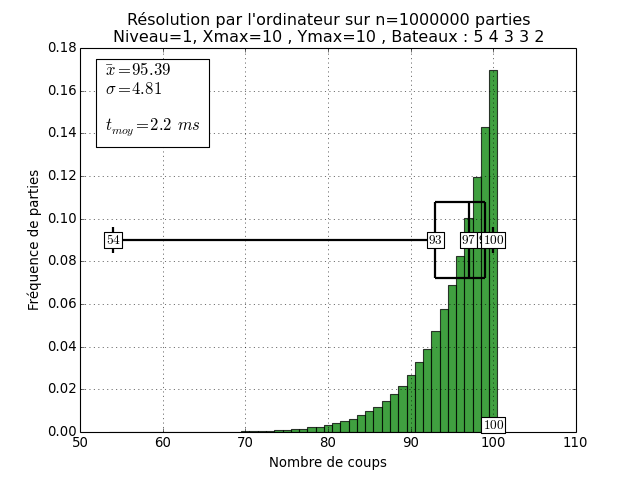
\includegraphics[scale=0.4]{./media/distrib_HAL_niveau=1_n=1000000.png}}
\end{center}
\end{frame}

\begin{frame}{Niveau 2 : tirs aléatoires + file}
Résultats sur $n=1\,000\,000$ parties :
\begin{center}
\fbox{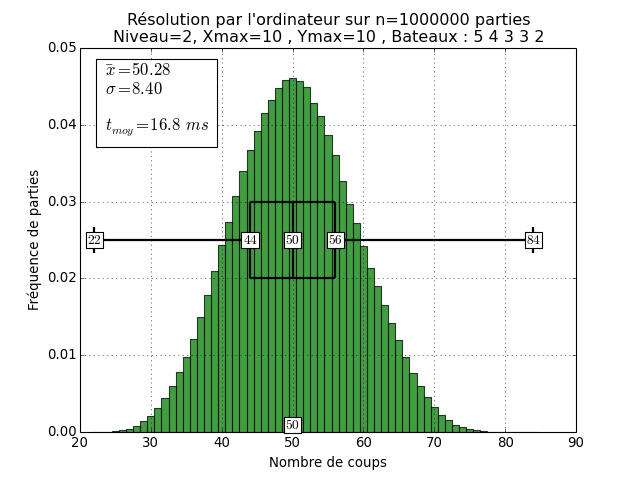
\includegraphics[scale=0.4]{./media/distrib_HAL_niveau=2_n=1000000.png}}
\end{center}
\end{frame}

\begin{frame}{Niveau 3 : cases noires + file}
Résultats sur $n=1\,000\,000$ parties :
\begin{center}
\fbox{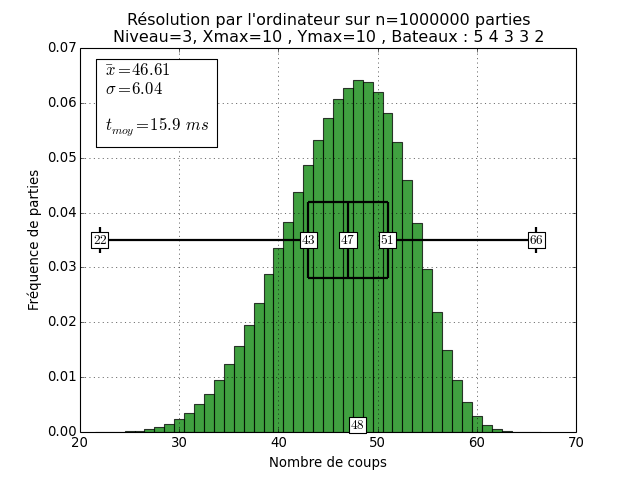
\includegraphics[scale=0.4]{./media/distrib_HAL_niveau=3_n=1000000.png}}
\end{center}
\end{frame}


\begin{frame}{Niveau 4(10) : échantillons de taille 10}
Résultats sur $n=100\,000$ parties :
\begin{center}
\fbox{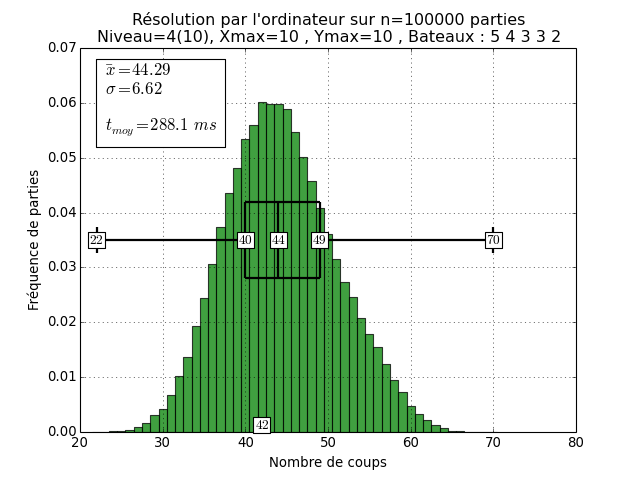
\includegraphics[scale=0.4]{./media/distrib_HAL_niveau=4(10)_n=100000.png}}
\end{center}
\end{frame}

\begin{frame}{Niveau 4(100) : échantillons de taille 100}
Résultats sur $n=10\,000$ parties :
\begin{center}
\fbox{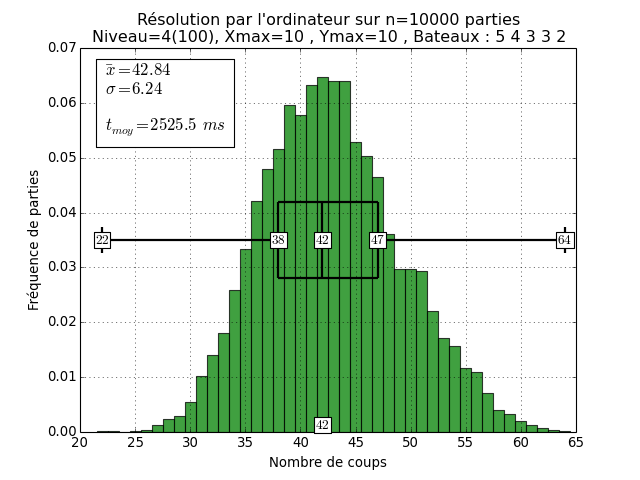
\includegraphics[scale=0.4]{./media/distrib_HAL_niveau=4(100)_n=10000.png}}
\end{center}
\end{frame}

\begin{frame}{Niveau 4(1000) : échantillons de taille 1000}
Résultats sur $n=1\,000$ parties :
\begin{center}
\fbox{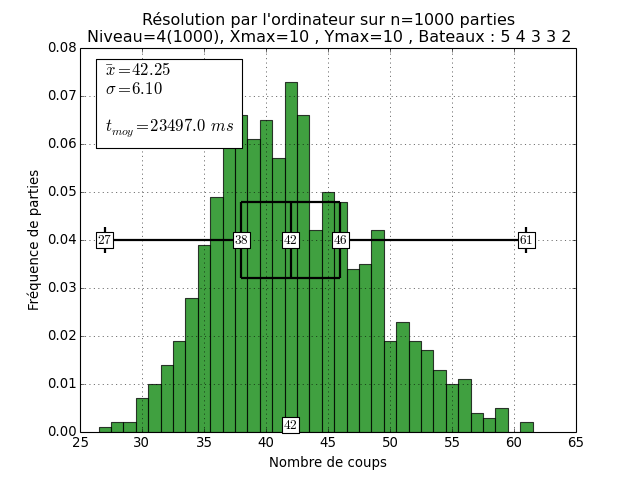
\includegraphics[scale=0.4]{./media/distrib_HAL_niveau=4(1000)_n=1000.png}}
\end{center}
\end{frame}

\begin{frame}{Niveau 4(10000) : échantillons de taille 10000}
Résultats sur $n=100$ parties :
\begin{center}
\fbox{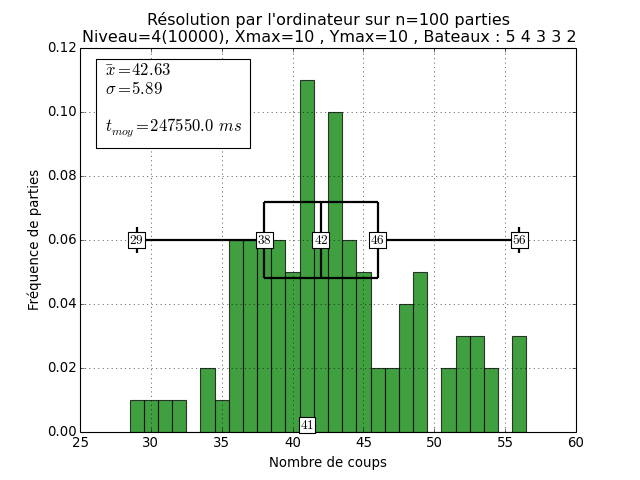
\includegraphics[scale=0.4]{./media/distrib_HAL_niveau=4(10000)_n=100.png}}
\end{center}
\end{frame}

\begin{frame}{Conclusion niveau 4}
\begin{center}
\begin{tabular}{|l|c|c|c|c|}
\hline
\no & 1 & 2 & 3 & 4\\
\hline
\texttt{nb\_echantillons} & 10 & 100 &  1\,000 & 10\,000\\
\hline
$n$ & 100\,000 & 10\,000 & 1\,000 & 100\\
\hline
$\conj x$ & 44,29 & 42,84 & 42,25 & 42,63\\
\hline
$\sigma$ & 6,62 & 6,24 & 6,10 & 5,89\\
\hline
$t_{moy}$ (en secondes)& 0,29 & 2,5 & 23,5 & 247\\
\hline 
\end{tabular}
\end{center}
\end{frame}

\begin{frame}
\begin{center}
\begin{tabular}{|l|l|c|}
\hline
\no & \texttt{nb\_echantillons} & Intervalle de confiance de $\mu$ \\
\hline
1 & 10 & $[44,25~;~44,33]$\\
\hline
2 & 100 & $[42,72 ~;~42,96]$\\
\hline
3 & 1\,000 & $[41,87~;~42,63]$\\
\hline
4 & 10\,000& $[41,48~;~43,78]$\\
\hline
\end{tabular}
\end{center}
\end{frame}


\begin{frame}{Niveau 5 : nombre local de bateaux}
Résultats sur $n=1\,000\,000$ parties :
\begin{center}
\fbox{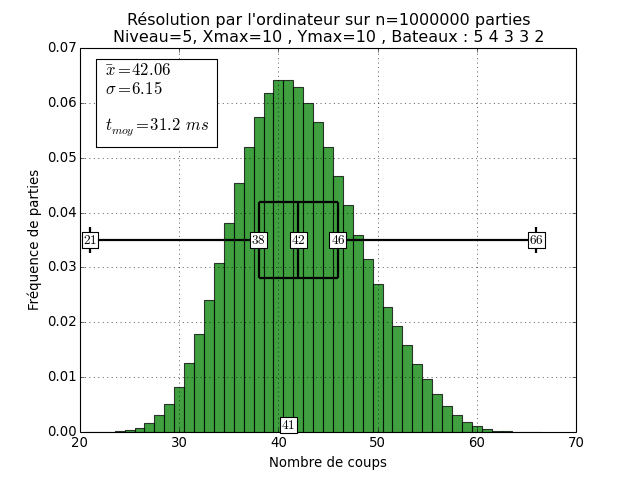
\includegraphics[scale=0.4]{./media/distrib_HAL_niveau=5_n=1000000.png}}
\end{center}
\end{frame}

\begin{frame}{Niveau 6(60) : tous les arrangements, seuil=60}
Résultats sur $n=10\,000$ parties :
\begin{center}
\fbox{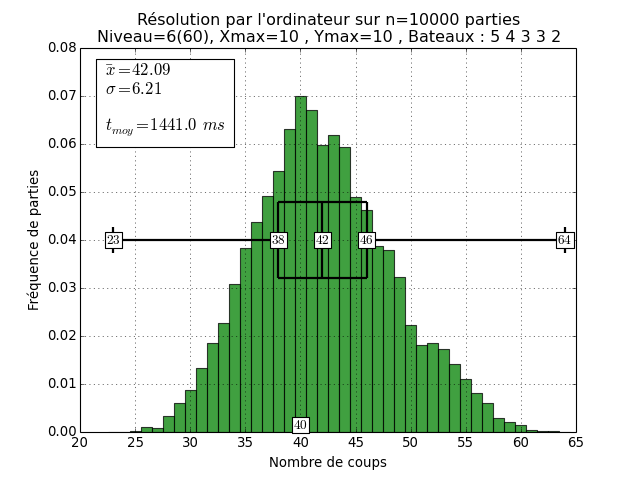
\includegraphics[scale=0.4]{./media/distrib_HAL_niveau=6(60)_n=10000.png}}
\end{center}
\end{frame}

\begin{frame}{Niveau 6(70) : tous les arrangements, seuil=70}
Résultats sur $n=1\,000$ parties :
\begin{center}
\fbox{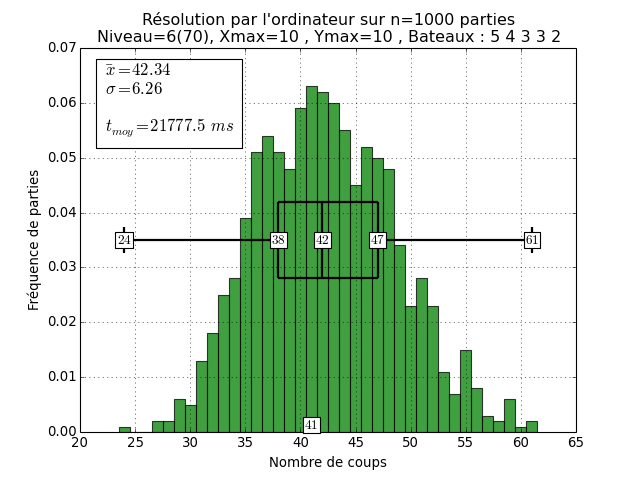
\includegraphics[scale=0.4]{./media/distrib_HAL_niveau=6(70)_n=1000.png}}
\end{center}
\end{frame}

\begin{frame}{Conclusion niveau 6}
\begin{center}
\begin{tabular}{|l|l|c|c|c|c|}
\hline
\no & Niveau & $n$ &  $\conj x$ & $\sigma$ & Intervalle de confiance\\
\hline
1 & 5 & 1\,000\,000 & 42,06 & 6,15 & $[42,05~;~42,07]$ \\
\hline
2 & 6(60) & 10\,000 & 42,09 & 6,21 & $[41,97~;~42,21]$\\
\hline
3 & 6(70) & 1\,000 & 42,34 & 6,26 & $[41,95~;~42,73]$\\
\hline
\end{tabular}
\end{center}
\end{frame}

\section{Le reste dont je n'aurai pas le temps de parler}
\begin{frame}{Interface console}
\begin{itemize}
\item Menu de choix de mode de jeu\pause
\item Étude statistique des algorithmes\pause
\item Affichages de la grille, et surlignage des bateaux
\end{itemize}
\end{frame}

\begin{frame}{Interface web}
\begin{itemize}
\item Script \texttt{cgi}\pause
\item Gestion d'un \texttt{canvas} et de la souris en JavaScript\pause
\item Sauvegarde des paramètres de la partie
\end{itemize}

\end{frame}

\begin{frame}{Interface en \texttt{tkinter}}
\begin{itemize}
\item Différentes fenêtres\pause
\item Placement des bateaux\pause
\item Illustration graphique de l'algorithme de résolution
\end{itemize}
\end{frame}

\section{Conclusion}
\begin{frame}
Un projet passionnant et prenant\pause

\medskip

Réalisé entièrement en solo\pause

\medskip

Un travail conséquent :\pause

\begin{itemize}
\item 4 mois et plus de 200 heures de travail intensif\\ \pause
\item 3500 lignes de code Python\\ \pause
\item 2000 lignes de \LaTeX pour le rapport\\ \pause
\item 2000  lignes de \LaTeX pour le diaporama\\ \pause
\end{itemize}
Et quelques nuits blanches de réflexion...
\end{frame}

\begin{frame}{}

\begin{center}
{\Huge Merci de votre attention}

\bigskip
Passons aux questions...


\end{center}
\end{frame}



\end{document}